%------------------ vorlage.tex ------------------------------------------------
%
% LaTeX-Vorlage zur Erstellung von Projektdokumentationen
% im Fachbereich Informatik der Hochschule Trier
%
% Basis: Vorlage 'svmono' des Springer Verlags
% Bearbeiter: Hermann Schloß, Christian Bettinger
%
%-------------------------------------------------------------------------------


%------------------ Präambel ---------------------------------------------------
\documentclass[envcountsame, envcountchap, deutsch]{i-studis}

\usepackage[utf8]{inputenc}

\usepackage[a4paper]{geometry}
\usepackage[english, ngerman]{babel}

\usepackage[pdftex]{graphicx}
\usepackage{epstopdf}

\usepackage{listings}

\usepackage[german, ruled, vlined]{algorithm2e}
\usepackage{amssymb, amsfonts, amstext, amsmath}
\usepackage{array}
\usepackage[skip=10pt]{caption}
\usepackage[usenames, dvipsnames]{color}
\usepackage[pdftex, plainpages=false]{hyperref}
\usepackage{textcomp}
\usepackage{tabularx}

\usepackage{bibgerm}
\bibliographystyle{geralpha}

\usepackage{makeidx}
\usepackage{multicol}
\makeindex

\pagestyle{myheadings}
\setlength{\textheight}{1.1\textheight}

\lstset{
	basicstyle=\scriptsize\ttfamily,
	commentstyle=\scriptsize\ttfamily\color{Gray},
	identifierstyle=\scriptsize\ttfamily,
	keywordstyle=\scriptsize\ttfamily,
	stringstyle=\scriptsize\ttfamily,
	tabsize=4,
	numbers=left,
	numberstyle=\tiny,
	numberblanklines=false,
	frame=single,
	framesep=3mm,
	framexleftmargin=7mm,
	xleftmargin=10mm,
	linewidth=144mm,
	captionpos=b,
}


%------------------ Manuelle Silbentrennung ------------------------------------
\hyphenation{Ele-men-tar-ob-jek-te ab-ge-tas-tet Aus-wer-tung House-holder-Matrix Least-Squares-Al-go-ri-th-men}


%------------------ Titelseite -------------------------------------------------
\begin{document}

\title{KI-gestützte Clusterung von studentischen Programmierlösungen zur Verbesserung automatisierter Feedbackprozesse}
\subtitle{AI-supported clustering of student programming solutions to improve automated feedback processes}

\author{Gregor Germerodt}

\supervisor{Prof. Dr. Michael Striewe}

\address{Trier}
\submitdate{07.07.2025}

%------------------ Projektart -------------------------------------------------
%\project{Bachelor-Teamprojekt}
\project{Bachelor-Abschlussarbeit}
%\project{Master-Projektstudium}
%\project{Master-Abschlussarbeit}
%\project{Seminar}
%\project{Hausarbeit}

\mytitlepage

%------------------ Vorwort, Kurzfassung, Verzeichnisse ------------------------
\frontmatter
\preface

Ein Vorwort ist nicht unbedingt nötig. Falls Sie ein Vorwort schreiben, so ist dies der Platz, um z.B. das Unternehmen vorzustellen, in der diese Arbeit entstanden ist, oder um den Personen zu danken, die in irgendeiner Form positiv zur Entstehung dieser Arbeit beigetragen haben.

Auf keinen Fall sollten Sie im Vorwort die Aufgabenstellung näher erläutern oder vertieft auf technische Sachverhalte eingehen.
								% Vorwort (optional)
\kurzfassung

In der Kurzfassung soll in kurzer und prägnanter Weise der wesentliche Inhalt der Arbeit beschrieben werden. Dazu zählen vor allem eine kurze Aufgabenbeschreibung, der Lösungsansatz sowie die wesentlichen Ergebnisse der Arbeit. Ein häufiger Fehler für die Kurzfassung ist, dass lediglich die Aufgabenbeschreibung (d.h. das Problem) in Kurzform vorgelegt wird. Die Kurzfassung soll aber die gesamte Arbeit widerspiegeln. Deshalb sind vor allem die erzielten Ergebnisse darzustellen. Die Kurzfassung soll etwa eine halbe bis ganze DIN-A4-Seite umfassen.

Hinweis: Schreiben Sie die Kurzfassung am Ende der Arbeit, denn eventuell ist Ihnen beim Schreiben erst vollends klar geworden, was das Wesentliche der Arbeit ist bzw. welche Schwerpunkte Sie bei der Arbeit gesetzt haben. Andernfalls laufen Sie Gefahr, dass die Kurzfassung nicht zum Rest der Arbeit passt.

\kurzfassungEN

The same in English.
							% Kurzfassung/Abstract
\tableofcontents										% Inhaltsverzeichnis
\listoffigures											% Abbildungsverzeichnis (optional)
\listoftables											% Tabellenverzeichnis (optional)
\lstlistoflistings										% Listings (optional)


%------------------ Kapitel ----------------------------------------------------
\mainmatter
\chapter{Einleitung und Problemstellung}

% Begonnen werden soll mit einer Einleitung zum Thema, also Hintergrund und Ziel erläutert werden.

% Weiterhin wird das vorliegende Problem diskutiert: Was ist zu lösen, warum ist es wichtig, dass man dieses Problem löst und welche Lösungsansätze gibt es bereits. Der Bezug auf vorhandene oder eben bisher fehlende Lösungen begründet auch die Intention und Bedeutung dieser Arbeit. Dies können allgemeine Gesichtspunkte sein: Man liefert einen Beitrag für ein generelles Problem oder man hat eine spezielle Systemumgebung oder ein spezielles Produkt (z.B. in einem Unternehmen), woraus sich dieses noch zu lösende Problem ergibt.

% Im weiteren Verlauf wird die Problemstellung konkret dargestellt: Was ist spezifisch zu lösen? Welche Randbedingungen sind gegeben und was ist die Zielsetzung? Letztere soll das beschreiben, was man mit dieser Arbeit (mindestens) erreichen möchte.

Für Lehrkräfte an Hochschulen oder Universitäten kann das Kontrollieren und Bewerten von studentischen Einreichungen je nach Menge zu einer großen Herausforderung werden. Gerade bei einer hohen Anzahl an Abgaben steigt der Korrekturaufwand erheblich, was den zeitlichen Rahmen für individuelles Feedback einschränken kann. Eine Untersuchung zeigte, dass das Kontrollieren und Bewerten von Arbeiten der Hauptfaktor für Arbeitsbelastung und Beeinträchtigung des Wohlbefindens ist (vgl. \cite{Jerrim.2021}). In der Informatik könnte es sich hier auf Programmieraufgaben beziehen. Dabei müssen Lehrkräfte konsistente Bewertungen abliefern, während jede Abgabe unterschiedliche Syntax und Semantik beinhalten kann.

Eine Lösung dieses Problems bieten etablierte Systeme zur automatischen Auswertung von Programmieraufgaben. Systematische Übersichtsarbeiten zeigen, dass viele Werkzeuge vorwiegend auf Unit-Tests oder statische Analysen setzen, was meist zu eher generischem Feedback führt (vgl. \cite{Messer.2023}). Die Hoschule Trier benutzt beispielsweise ASB - Automatische Software-Bewertung\footnote{https://www.hochschule-trier.de/informatik/forschung/projekte/asb}. Nachdem hierbei Studierende die von der Lehrkraft gestellte Aufgabe bearbeitet haben, können sie online ihre Lösungen hochladen. Das Programm prüft danach nach statischen Kriterien, ob z. B. alle benötigen Dateien hochgeladen wurden, ob sie der Namenskonvention entsprechen, etc. Daraufhin wird das hochgeladene Programm mit Testdaten ausgeführt und geprüft, ob die zu erwarteten Ergebnisse ausgegeben werden. Sollte das nicht der Fall sein, wird eine Fehlermeldung ausgegeben, dass das Programm oder bestimmte Module nicht erwartungsgemäß funktionieren. 

Das erzeugte Feedback solcher statischen Systeme dient zur Orierentierung, jedoch weniger zur Fehlersuche, da es recht allgemein gehalten ist. Um die Feedbackgenerierung zu verbessern könnten KI-gestütze Verfahren eingesetzt werden. Damit befassten sich beispielsweise die Autoren der wissenschaftlichen Arbeiten \dots (Hier Quellen einfügen und erläutern).

Dazu wurde in dieser Arbeit versucht, einen Schritt vor der Feedbackgenerierung zu entwickeln. Er befasst sich mit der KI-gestützten Clusterung studentischer Programmierlösungen. Dieser Ansatz ermöglicht es für mehrere Einreichungen ein gemeinsames Feedback zu generieren, indem sie nach Ähnlichkeit in Bezug auf Syntax und Semantik geclustert bzw. gruppiert werden. Weiterführende Prorgamme oder auch Lehrkräfte könnten dann einen Kandidat pro Cluster wählen, Feedback erzeugen und dieses an alle anderen Teilnehmer des Clusters weiterleiten. Dies könnte eine erhebliche Zeitersparnis zur Folge haben und weiterhin mehr Spielraum für präziseres individuelles Feedback ermöglichen. 
\chapter{Theoretische Grundlagen}

\section{Künstliche Intelligenz}
Künstliche Intelligenz (KI) bezeichnet die Wissenschaft und Technik der Entwicklung von Maschinen, die Aufgaben ausführen können, für die normalerweise menschliche Intelligenz erforderlich ist (Russell \& Norvig, 2021, S. 1). Der Mensch hat sich damit Systeme geschaffen, um die Kapazitäten menschlicher Intelligenz für bestimmte Aufgaben zu schonen oder zu erweitern. Dabei übernimmt die KI den Teil der Automatisierung monotoner Arbeit, also jenen Part, der durch menschliches Handeln erwiesenermaßen fehleranfällig ist, um konsistente Ergebnisse bereitzustellen. Automatisierung bedeutet in diesem Zusammenhang, dass Maschinen bestimmte Entscheidungs- und Handlungsprozesse eigenständig durchführen, ohne dass eine Person direkt in jeden einzelnen Schritt eingreifen muss. Während sich solche Systeme ursprünglich vor allem in der industriellen Fertigung etablierten, stellt sich zunehmend die Frage, wie sich vergleichbare Konzepte auf andere Bereiche übertragen lassen, wie etwa auf das Bildungswesen und hier speziell auf die Bewertung und Rückmeldung (Feedback) zu studentischen Programmierlösungen. Wie kann eine intelligente Automatisierung Lehrkräfte dabei unterstützen, qualitativ hochwertiges und individualisiertes Feedback zu generieren, ohne jede Lösung einzeln manuell prüfen zu müssen?

In dieser Arbeit wird KI anhand verschiedener Open-Source-Bibliotheken genutzt. Das System kombiniert mehrere KI-Techniken wie
\begin{itemize}
    \item Deep Learning - ein Teilbereich des Machine Learnings (ML), der künstliche neuronale Netze mit vielen Schichten verwendet, um komplexe Muster in Daten zu erkennen,
    \item Unsupervised Machine Learning - ein Verfahren, bei denen Modelle ohne beschriftete Trainingsdaten Muster oder Strukturen in den Daten erkennen, z.B. durch Clustering, und
    \item verschiedene Machine Learning Methoden, bei denen Computer aus Beispieldaten eigenständig Muster und Zusammenhänge erkennen, um daraus Vorhersagen oder Entscheidungen abzuleiten.
\end{itemize}
Das Zusammenspiel dieser Methoden führt letztlich zur Unterstützung der Lehrkräfte zur Feedbackgenerierung, was in den Ergebnissen zu sehen sein wird.

\section{Stand der Technik}
Inspiration für diese Arbeit wurde aus aktuellen Werken entnommen, wie Orvalho et al. (2022), die mit InvAASTCluster ein Verfahren zur Clusterung von Programmierlösungen mittels dynamischer Invarianten-Analyse vorstellen (vgl. \cite{Orvalho.28.06.2022}); aus Paiva et al. (2024) die AsanasCluster, ein inkrementelles k-means-basiertes Verfahren, zur Clusterung von Programmierlösungen für automatisiertes Feedback entwickelt haben (vgl. \cite{Paiva.2024}); und Tang et al. (2024) die Large Language Models\footnote{auf Textdaten trainierte KI-Modelle, die natürliche Sprache verarbeiten und generieren} (LLMs) und Clustering kombinieren, um personalisiertes Feedback in Programmierkursen zu skalieren (vgl. \cite{Tang.21.10.2024}).

Diese Quellen und weitere Recherche dienten zum Kennenlernen und zum späteren Einbinden von Algorithmen, die aufgrund ihrer besonderen Eignung zur Clusterung von Programmieraufgaben besonders herausstachen, wie 
\begin{itemize}
    \item k-means - eine Methode zur Aufteilung von N Beobachtungen in k Cluster, wobei jede Beobachtung zu dem Cluster mit dem nächstgelegenen Mittelwert gehört, der als Prototyp des Clusters dient, und
    \item hdbscan - eine Erweiterung des Density-Based Spatial Clustering of Applications with Noise (DBSCAN) Algorithmus, indem es eine Hierarchie von Clustern aufbaut und die stabilen Cluster über unterschiedliche Dichteebenen hinweg extrahiert,
\end{itemize}
Weiterhin wurden Verfahren eingebunden die hochdimensionale Vektoren in ihren Dimensionen reduzieren, um sie für weiterführende Prozesse wie z. B. zur Clusterung und Visualisierung der Daten nutzbar zu machen. In dieser Arbeit wurden
\begin{itemize}
    \item Principal component analysis (PCA) - ein Verfahren zur Projektion hochdimensionaler Daten in einen lineareren Unterraum mit geringerer Dimension, indem neue Achsen, entlang derer die Daten am stärksten streuen, berechnet werden und stellt die Daten entlang dieser Achsen dar,
    \item t-distributed stochastic neighbor embedding (t-SNE) - ein Verfahren zur Visualisierung hochdimensionaler Daten, indem es berechnet wie ähnlich Punkte zu ihren Originaldaten sind, um sie entsprechend weit auseinander oder nahe zusammen zu platzieren, und
    \item Uniform Manifold Approximation and Projection (UMAP) - ein Verfahren welches Topologie und Geometrie nutzt, um skalierbare, strukturtreue EIinbettungen in niedrigere Dimensionen zu erreichen.
\end{itemize}


\section{Relevanz von KI für Lehrkräfte}
Eine Studie des MDPI-Journals ergab, dass 92 \% der Lehrkräfte mit KI vertraut sind, und über 54 \% gaben an, KI bei administrativen Aufgaben, wie Notengebung oder Unterrichtsplanung zu nutzen. Laut Technikakzeptanzmodell (TAM) fördert die wahrgenommene Nützlichkeit (Perceived Usefulness, PU) die Verwendung von KI im Unterricht (vgl. \cite{}).

Eine Springer-Studie zeigt, dass KI-Tools die Unterrichtsgestaltung erleichtern und Inhalte ansprechender machen - was Selbstwirksamkeit, Engagement und Motivation der Lehrkräfte steigert (vgl. \cite{}).

Feldstudien mit intelligenten Assistenzsystemen im K-12-Bereich (etwa durch Lumilo-Smartglasses) verdeutlichten, dass KI von Lehrkräften als Ideenquelle und Entscheidungsunterstützung wahrgenommen wird, statt als Ersatz

% Methodik
% Aufgrund der weltweiten Etablierung und der Bereitstellung von Bibliotheken die die obigen KI-Techniken bereitstellen, wurde für die Programmierung des Systems Python als Programmiersprache benutzt. Darüber hinaus zeichnet sich Python durch eine einfache, lesbare Syntax und eine aktive Entwickler- und Forschungsgemeinschaft aus, was die Entwicklung, Erweiterung und Wartung des Systems erleichtert.
\chapter{Vorgehensweise und Implementierung}

\section{Themenfindung}
Die zunehmende Digitalisierung und der technologische Fortschritt eröffnen vielfältige Einsatzmöglichkeiten für Methoden der künstlichen Intelligenz (KI). Besonders im Bildungsbereich entsteht dadurch die Chance, Prozesse zu optimieren und Lehrkräfte bei Routineaufgaben zu entlasten.

Vor diesem Hintergrund wurde das Thema dieser Arbeit gewählt. Ziel ist es, das Potenzial von KI-gestützten Verfahren im Kontext der automatisierten Auswertung studentischer Programmierlösungen zu untersuchen. Durch die Clusterung ähnlicher Lösungen können neue Ansätze für Feedbackprozesse entwickelt werden, die eine effizientere und gezieltere Betreuung von Studierenden ermöglichen.


\section{Recherche und Vorbereitung}
Zu Beginn wurden diverse Quellen herausgesucht, die sich im Rahmen dieses Themas bewegen. Besonders oft stach dabei der k-Means Algorithmus heraus oder wie dieser als Grundlage für erweiternde Algorithmen wie den InvAASTCluster (vgl. \cite{Orvalho.28.06.2022}) oder AsanasCluster (vgl. \cite{Paiva.2024}) benutzt wurde, um bessere Ergebnisse zu liefern. Anhand eines Rankings wurde die Relevanz der Quellen festgelegt, um das weitere Vorgehen einzugrenzen.

Andere Methoden wie der Caliński-Harabasz Index oder der Silhouette Score wurden erwähnt, die zur Evaluation des Clusterings dienen. Es wurde klar, dass der Verlauf von studentischen Programmierlösungen bis zu nutzbaren Daten zur Feedbackgenerierung ein mehrschrittiger Prozess ist.

Der folgende Abschnitt, beschreibt die Entstehung des Programms bzw. einer Pipeline, die die benötigten Prozessschritte beeinhaltet, um dies zu erreichen.


\section{Implementierungsverlauf}
\subsection{Erster Implementierungsabschnitt}
Um einen mehrschrittigen Prozess zu vereinen, eignete sich das Prinzip einer Pipeline, in der nacheinander Algorithmen ablaufen, dessen Eingabewerte vom vorherigen Algorithmus abhängen und dessen Ausgabewerte dem Nächsten folglich wieder als Eingabe dienen.


\subsubsection*{Dateien laden}
Als erstes musste es eine Möglichkeit geben die Java-Dateien der studentischen Programmierlösungen einlesen zu können. Diese wurden als Datensätze durch den betreuenden Prof. Dr. Striewe bereitgestellt.

Der Datensatz an denen das Programm fortlaufend getestet wurde, bestand aus mehreren Überordnern und final aus drei Java-Dateien und einer Text-Datei, welche den Studierenden vorgegeben waren und vervollständigt werden mussten. Jedoch soll die Menge der Java-Dateien keine überwiegende Rolle spielen.

Das Programm musste also in der Lage sein Ordner zu durchsuchen und Java-Dateien zu erkennen. Dies ermöglichte eine Methode des ersten implementierten Moduls \texttt{data\_loader.py}. Es extrahierte Quellcode-Text und speicherte pro Datei Code-Schnipsel (Code Snippets) in eine Liste und gab diese an die Pipeline zurück.

Anfangs entstanden durch problematische Zeichen innerhald der Java-Dateien Fehlermeldungen, welche jedoch einfachheitshalber ignoriert werden.


\subsubsection*{Vektorrepräsentation}
Als nächstes folgte ein Modul zum einbetten dieser Code Snippets bzw. zum dessen repräsentieren durch hochdimensionale Vektoren. Dies war notwendig um sie für Clustering-Algorithmen vorzubereiten. 

Dafür wurde das Modul \texttt{embedding\_model.py} erstellt, welches vortrainierte Sprachmodelle aus der Transformers-Bibliothek\footnote{\url{https://huggingface.co/docs/transformers}} von Python (hier CodeBERT) und passende Tokenizer, die den Code vorbereitend für den Transformer in Tokens zerlegt, importiert.

Anhand einer Methode werden die Code Snippets in numerische Vektoren umwandelt (Embeddings). Alle enstandenen Embeddings wurde anschließend jeweils an die Pipeline zurückgegeben und in eine Liste abgespeichert.


\subsubsection*{Clustering}
Nun mussten die Embeddings geclustert werden. Das entsprechend erstellte Modul \texttt{clustering\_engine.py} importierte dafür die beiden Cluster Algorithmen k-Means aus der scikit-learn Bibliothek\footnote{\url{https://scikit-learn.org/stable/modules/generated/sklearn.cluster.KMeans.html}} für maschinelles Lernen und HDBSCAN aus der separaten HDBSCAN Python-Bibliothek\footnote{\url{https://hdbscan.readthedocs.io/en/latest/api.html\#hdbscan.hdbscan.HDBSCAN}}. An die Pipeline werden schließlich mit Markierungen (Labels) versehene Cluster zurückgegeben.


\subsubsection*{Evaluationsmetriken}
Anschließend wurde ein Evaluationsverfahren eingebaut, um die Qualität der Cluster zu bewerten. Dafür wurde das Modul \texttt{evaluation\_metrics.py} implementiert. Darin wird jeder Cluster nach den Evaluationsmetriken Silhouette Score\footnote{\url{https://scikit-learn.org/stable/modules/generated/sklearn.metrics.silhouette_score.html}}, Caliński-Harabasz Index\footnote{\url{https://scikit-learn.org/stable/modules/generated/sklearn.metrics.calinski_harabasz_score.html}} und den Davies-Bouldin Index\footnote{\url{https://scikit-learn.org/stable/modules/generated/sklearn.metrics.davies_bouldin_score.html}} getestet, welche ebenfalls aus der scikit-learn Bibliothek importiert wurden. Zurückgegeben wird ein Dictionary mit den drei Zahlenwerten der Evaluationsmetriken.


\subsubsection*{Tests, Optimierungen und Dokumentation}
Jedes implementierte Modul wurde einzeln getestet. Dazu wurden das Ergebnis und die Zeit, welche für den jeweiligen Prozessschritt notwendig waren durch print-Anweisungen ausgegeben. Dabei stellte sich heraus, dass Embedding und besonders Imports relativ viel Zeit in Anspruch nahmen.

Da die zu testenden Datensätze teilweise aus mehreren hunderten Dateien bestanden, wurde dazu caching der Embeddings eingeführt, um das Testen des Zusammenspiels der einzelnen Module zu beschleunigen. Versuche die Imports durch lazy loading zu beschleunigen waren in diesem Fall nur geringfügig merkbar.

Des Weiteren wurde eine Requirements.txt-Datei erstellt. Diese beeinhaltet sämltiche Information über die aktuell im Projekt benutzen Versionen der importierten Bibliotheken. Sie sorgt, dass für andere Nutzende gleiche Bedingungen wie auch in der Entwicklung herrschen, um ein lauffähiges Programm zu gewährleisten.

Die noch später hinzugefügte Datei HowToInstall.txt dient zusätzlich als Schritt-für-Schritt-Anleitung. Weiterhin wurde eine config.yaml-Datei hinzugefügt. Diese diente als zentrale Ansprechquelle der Pipeline für Parameter.


\subsubsection*{Dimensionsreduktion}
Zu diesem Zeitpunkt war ein Visualisierungs-Modul geplant, um die Clusterungen sichtbar zu machen, doch bevor es sinnvoll eingesetzt werden konnte, wurde noch ein weiterer Prozessschritt eingebunden, das Dimensionsreduktionsverfahren bzw. dessen Algorithmen. Das entsprechende Modul \texttt{dimensionality\_reducer.py} importiert auch hier Algorithmen aus der scikit-learn Bibliothek, die Principal Component Analysis (PCA)\footnote{\url{https://scikit-learn.org/stable/modules/generated/sklearn.decomposition.PCA.html}} und t-Distributed Stochastic Neighbor Embedding (t-SNE)\footnote{\url{https://scikit-learn.org/stable/modules/generated/sklearn.manifold.TSNE.html}}. Der dritte Algorithmus Uniform Manifold Approximation and Projection (UMAP)\footnote{\url{https://umap-learn.readthedocs.io/en/latest/}} stammt aus der eigenständigen UMAP-learn Bibliothek. 

Dieser Prozessschritt findet zwischen Embedding und Clustering statt. Er reduziert die Embeddings bzw. die hochdimensionalen Vektoren in ihren Dimensionen (hier zu 2D oder 3D), welche danach zur Clusterung weitergereicht und dadurch auch besser als menschlicher Betrachter in einem Diagramm beobachtet werden können.


\subsubsection*{Visualisierung}
Schließlich wurde noch das Modul \texttt{cluster\_plotter.py} implementiert, welches anhand der dimensionsreduzierten Embeddings und der aus dem Clustering hervorgegangenen Labels ein statisches Diagramm (engl. plot) in einem separatem Fenster erstellt (Beispiel-Clusterung in Abbildung \ref{abb:E-CD}). Hierfür wurden aus der Matplotlibs Bibliothek die Plotting-Module pyplot\footnote{\url{https://matplotlib.org/stable/api/pyplot_summary.html}} und \texttt{mpl\_toolkits.mplot3d}\footnote{\url{https://matplotlib.org/stable/gallery/mplot3d/2dcollections3d.html\#sphx-glr-gallery-mplot3d-2dcollections3d-py}} importiert, die für 2D- und 3D-Visualisierung (falls gewünscht) zuständig sind.

Die zuvor erstellten Module gleichten sich durch ihre einheitlichen Klassenstruktur, da jedoch für dieses Modul keine Zwischenspeicherung von Zuständen anhand einer Instanz notwendig war, wurden dessen Methoden statisch definiert.


\subsubsection*{Pipeline}
Die Pipeline besteht zu diesem Zeitpunkt aus folgendem Ablauf:

\textbf{Daten laden} $\rightarrow$ \textbf{Einbetten} $\rightarrow$ \textbf{Dimensionen reduzieren} $\rightarrow$ \textbf{Clustern} $\rightarrow$ \textbf{Evaluieren} $\rightarrow$ \textbf{Visualisieren}

\begin{figure} %[hbtp]
	\centering
	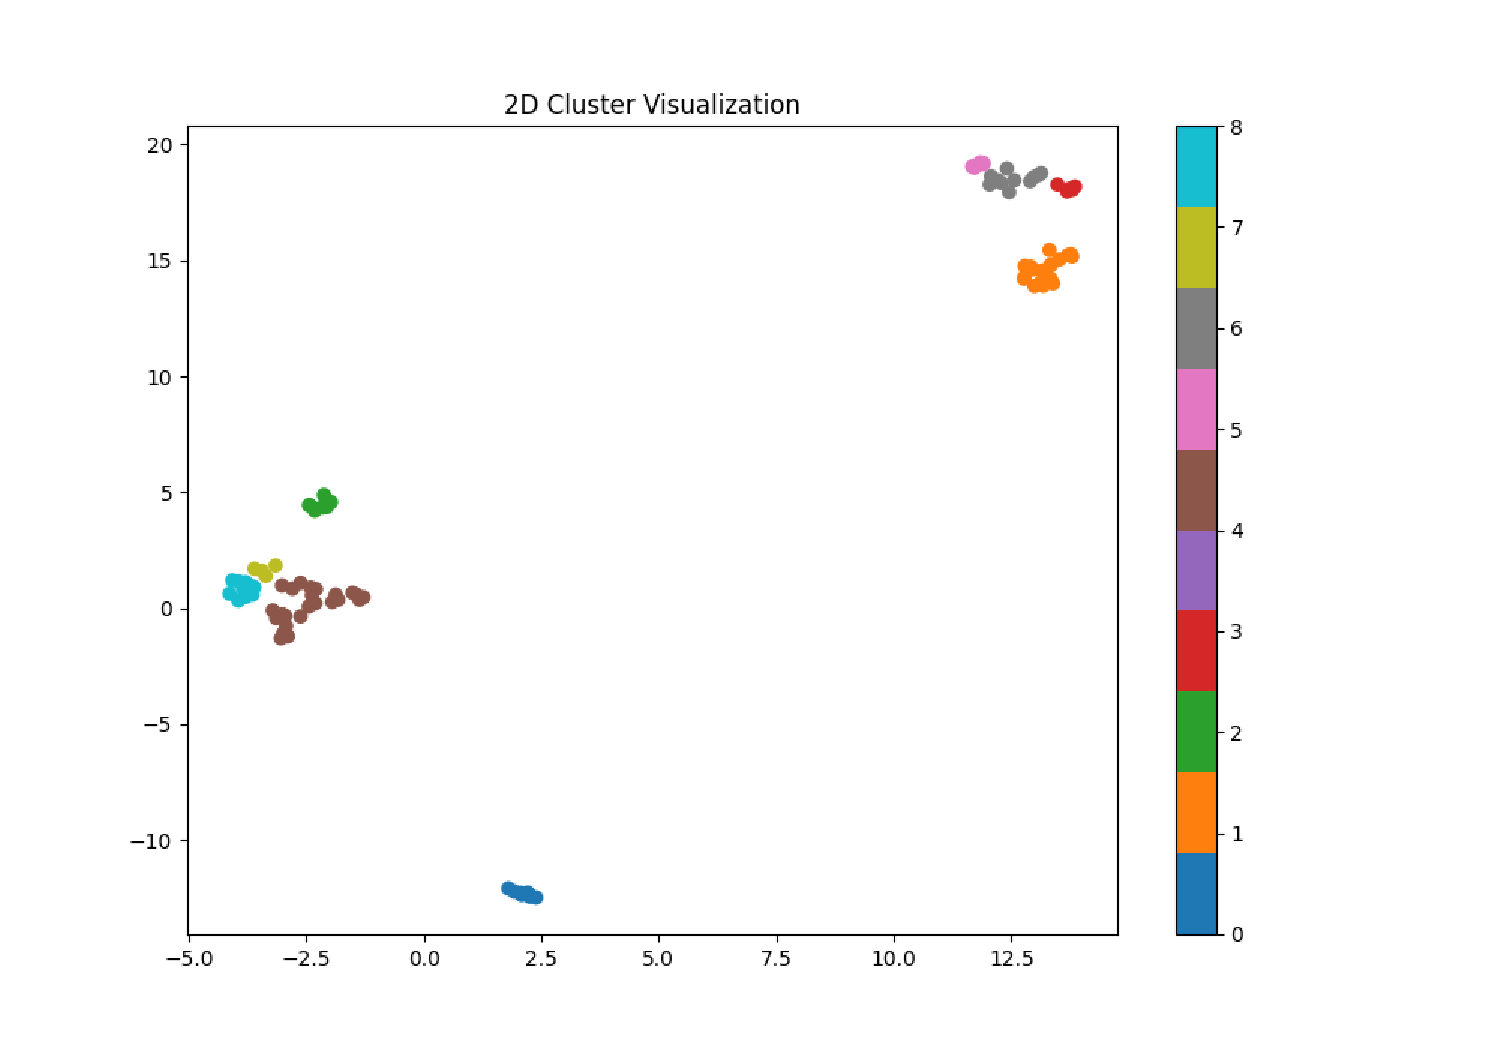
\includegraphics[width=0.8\textwidth]{images/Erstes Clustering-Diagramm.pdf}
	\caption{Zweidimensionales Clustering-Diagramm einer Clusterung von 147 Java-Dateien. Die unterschiedlichen Farben kennzeichnen die Zugehörigkeit der Punkte zu einem Cluster. Am rechten Rand sind die benutzten Farben in einer Farbskala angeordnet.}
	\label{abb:E-CD}
\end{figure}


\subsection{Zweiter Implementierungsabschnitt}
\subsubsection*{Interaktive Diagramme}
In Abbildung \ref{abb:I-CD} sind zwar farbige Punkte in unterschiedlicher Anzahl pro Cluster zu erkennen, jedoch wurden keine Labels angezeigt, die Informationen über die Punkte anzeigen sollten. Als vorbereitender Schritt für weiterführende Prozesse zur automatischen Feedbackgenerierung, müssen sie zumindest zum Testen visuell zuordenbar sein.

Aus diesem Grund wurde ein weiteres Modul zur Visualisierung implementiert. Das entstandene Modul \texttt{interactive\_plot.py} nahm dafür wieder Embeddings, Labels und zustätzlich noch den Namen der aktuellen Java-Datei entgegen, die im \texttt{data\_loader.py}-Modul gespeichert wurde.

Dazu wurden aus der Python-Bibliothek die Module Pandas\footnote{\url{https://pandas.pydata.org/docs/}} und Plotly Express\footnote{\url{https://plotly.com/python/plotly-express/}} importiert, die einerseits zur Erstellung von Tabellenstrukturen (DataFrames) und andererseits für einfache und interaktiave Diagramme zuständig sind. Ausgeführt, öffnete sich ein Fenster im Webbrowser mit einem von der Gestalung her ähnlichem Diagramm wie in der statischen Variante (\ref{abb:E-CD}).

\begin{figure} %[hbtp]
	\centering
	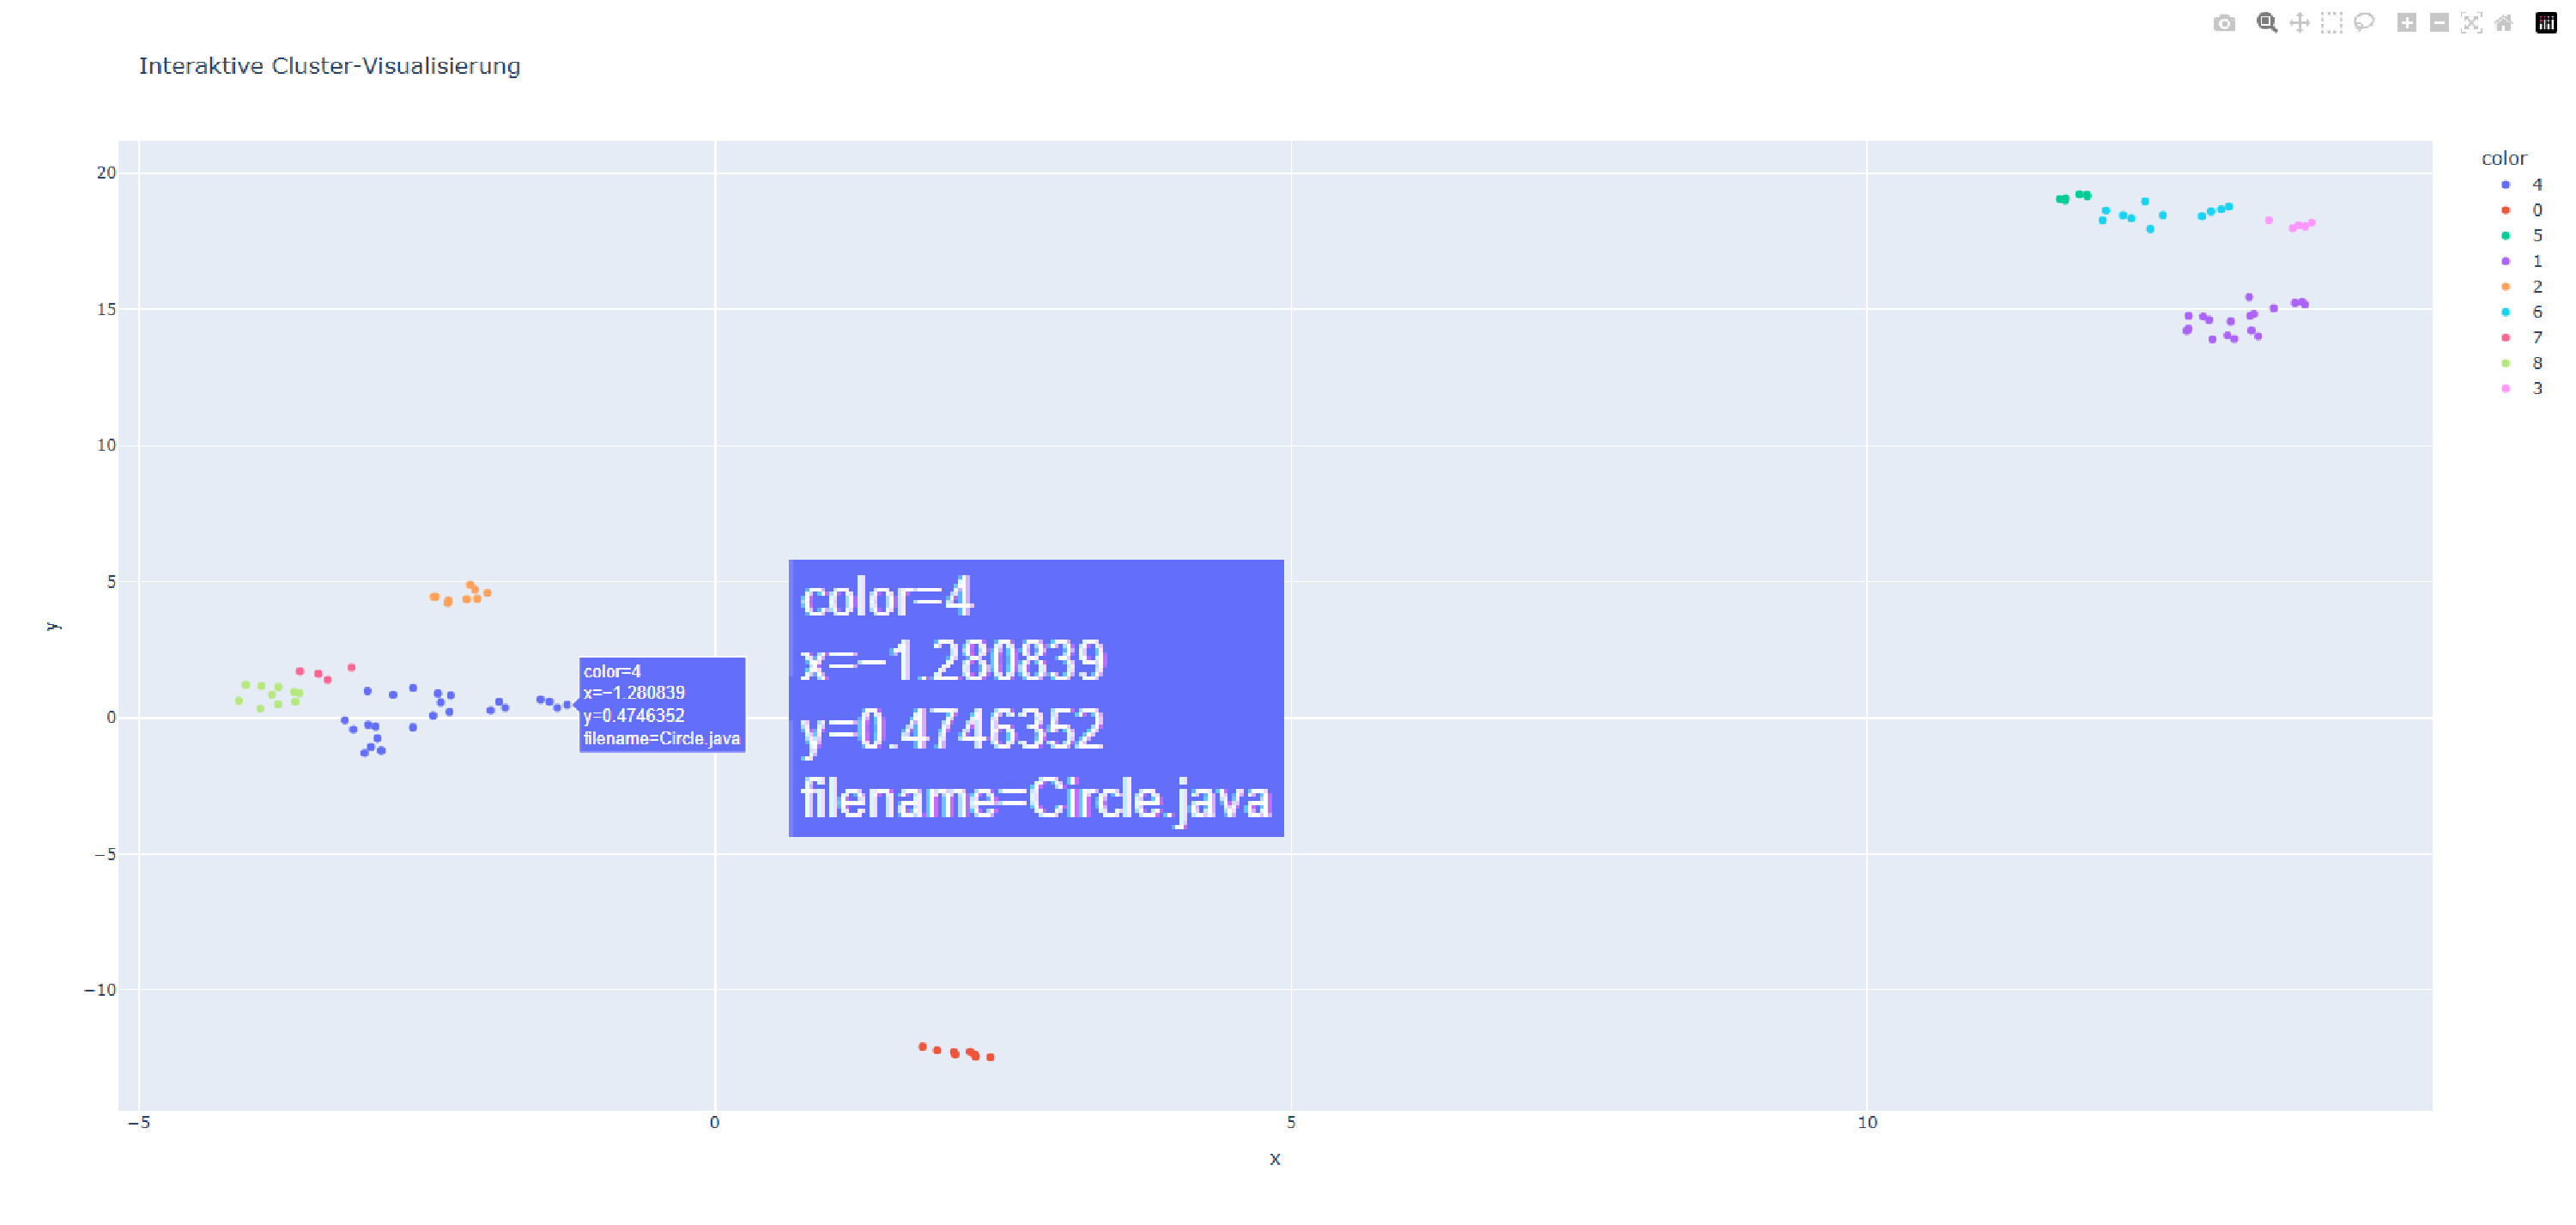
\includegraphics[width=1.0\textwidth]{images/Interaktives Clustering-Diagramm.pdf}
	\caption{Interaktives Clustering-Diagramm einer Clusterung von 147 Java-Dateien. Durch das Halten der Maus über die Punkte werden Informationen über sie angezeigt (im Bild wiederholt vergrößert dargestellt). Am rechten Rand sind die Mengen der Cluster angezeigt.}
	\label{abb:I-CD}
\end{figure}


\subsubsection*{Probleme bei der Cluster-Konsistenz und getroffene Maßnahmen}
Beim mehrmaligen Austesten verschiedener Dateimengen und Überprüfen der ausgegeben Punkte, fiel auf, dass Cluster bei größeren Datenmengen nicht mehr konsistent sind, obwohl akzeptable Ergebnisse im Evaluationsmetriken erreicht wurden. Genauer genommen wurden vereinzelt unterschiedliche Dateien in einem gemeinsamen Cluster platziert (gezeigt in \ref{abs:C-u-D-i-e-D} in Abschnitt Forschungsergebnisse). So kamen beispielsweise Point.java-Dateien in einem Cluster mit sonst nur Circle.java-Dateien vor.

Da Clustering-Algorithmen nach ähnlicher Syntax und Semantik clustern, kann solch ein Verhalten durchaus vor kommen, ist hier jedoch nicht von praktischen Nutzen. Andererseits könnten ebenso Fehler in den Algorithmen oder Inkonsistenzen in den gegebenen Datensätzen die fehlerhafte Clusterung verursachen. Selbst Dateien die abhängig von der gestellten Aufgabe zu den Einreichungen bereits gegeben waren, nicht bearbeitet werden sollten und überall identisch waren, wurden in verschiedenen Clustern angeordnet.

Als erste Maßnahme gegen dieses Problem, wurden die nicht zu bearbeitenden Dateien ignoriert, indem nicht mehr allgemein nach.java-Dateien gesucht wird, sondern nur noch nach bestimmten Namen. 

Im weiterem Verlauf wurde zudem in der Pipeline eine Schleife ergänzt, die die Prozesse ab Embedding bis zur Visualisierung für die gewünschten, in der Konfigurationsdatei festgelegten Namen bzw. Java-Dateien wiederholt. Dadurch werden gemischte Cluster verhindert und für jede unterschiedene Java-Datei ein Diagramm erstellt.

Weiterhin ist beim Testen einer niedriger Anzahl von Dateien (\(n \leq 4\)) aufgefallen, dass der Embedding-Algorithmus nicht mehr funtkioniert, jedoch ist solche eine Clusterung ohnehin nicht von Nutzen.


\subsubsection*{Experimentierungspipeline}
Um die Evaluationsmetriken einfach testen zu können, wurde eine separate Experimentierungspipeline erstellt. Der Vorteil bestand darin, dass die verschiedenen Kombinationen der Dimensionsreduktions- und Clustering-Algorithmen mit ihren Parametern über Dictionaries innerhalb der Pipeline definiert wurden. Die Evaluationsergebnisse wurden anschließend in einer CSV-Datei im Projektverzeichnis festgehalten.

In den Tabellen \ref{tab:EI-EV-20} und \ref{tab:EI-EV-160} im Abschnitt Forschungsergebnisse wurde gezeigt, welche Algorithmen-Kombination für verschiedene Dateimengen geeignet sind.


\subsubsection*{Visuelle Erweiterung}
Um den Punkten im Diagramm mehr Informationen entnehmen zu können, wurde neben den Dateinamen nun noch der Name des Einreichungsordners hinzugefügt. Da die erreichten Punktzahlen der Einreichungen Teil des Ordnernames sind, konnten die Clusterungen jetzt besser nachvollzogen und überprüft werden. Weiterhin wurde das \texttt{interactive\_plot.py}-Modul um die Option das Diagramm als dreidimensionale Umgebung darzustellen erweitert. Sollten mehrere Cluster im 2D-Diagramm aufeinanderliegen, so kann die dritte Achse bessere Einsicht gewährleisten.


\subsection{Dritter Implementierungsabschnitt}
\subsubsection*{Konkatenation gesuchter Dateien}
Auch wenn für jede durch Namen getrennte Art Datei ein separates Diagramm erstellt wird, besteht die Möglichkeit dass die vollständige Einreichung bzw. Lösung zu den gestellten Aufgaben gesamt betrachtet werden sollte, da es sonst zu verminderter Information führen könnte. Um die Dateien als ein Ganzes zu betrachten, wurde das \texttt{data\_loader.py}-Modul um eine Konkatenations-Funktionalität ergänzt. Die entstandene Methode konkateniert alle gesuchten Java-Dateien eines Einreichungsordners. Der im Diagramm gezeigte Dateiname eines Punktes, setzt sich nun aus den konkatenierten Namen der Dateien zusammen. Die Schleife in der Pipeline die die Prozessschritte für jede gesuchte Art Datei wiederholte, wurde daraufhin entfernt.


\subsubsection*{Probleme bei der Cluster-Visualisierung und Punktzuordnung}
Theoretisch wäre das Programm in der Lage, Embeddings ohne Dimensionsreduktionsalgorithmen zu verarbeiten. Zum Testen wird jedoch weiterhin eine geeignete Visualisierung verwendet, bei der allerdings durch die Anzeige der Ordnernamen pro Punkt ein weiteres Probleme auffiel. So werden konkatenierte Dateien in einen Cluster gesteckt, dessen Ordnernamen sich durch stark variierende Punktzahlen unterscheiden, wie in Abbildung \ref{abb:C-40-K-Pg} zu sehen ist. Auch hier kann solch ein Verahlten durchaus vorkommen, ist aber nicht von praktischen Nutzen, da sich das zu generierende Feedback nach den erreichten Punktzahlen unterscheiden sollte. 

\begin{figure} %[hbtp]
	\centering
	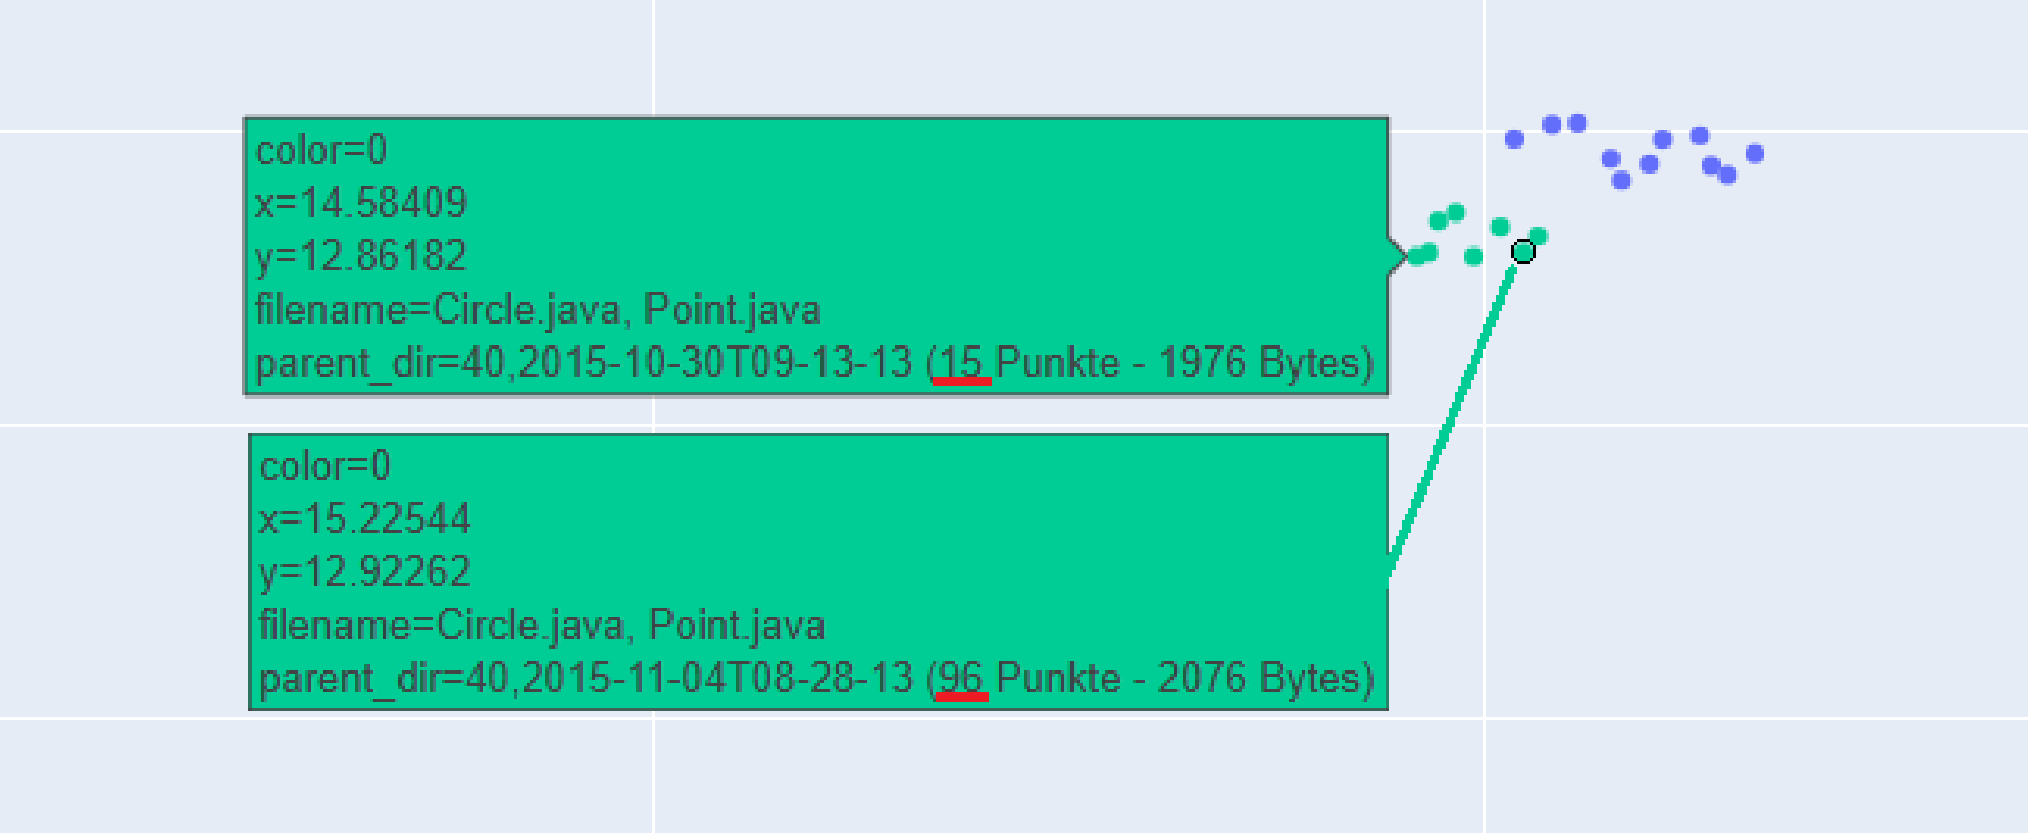
\includegraphics[width=1.0\textwidth]{images/Clusterung - 40 - Konkateniert - Punktzahl gemischt.pdf}
	\caption{Interaktives Clustering-Diagramm einer Clusterung von 80 bzw. 40 konkatenierten Java-Dateien. Die rote Unterstreichung zeigt das Problem gemischert Cluster mit unterschiedlichen Punktzahlen.}
	\label{abb:C-40-K-Pg}
\end{figure}


\subsubsection*{Punktzahlenintervalle}
Um diesem Problem entgegenzuwirken, wurde erneut die Vorgehensweise der wiederholten Prozessschritte mittels einer Schleife angewendet, indem nach Ebenen bzw. Punktzahlenintervallen (Score-Bins) geclustert wird. Es können beliebig viele Intervalle definiert werden (z. B. 0-49, 50-79, 80-89, 90-100), um das Clustering weiter zu präzisieren. Dafür wurde dem \texttt{data\_loader.py}-Modul eine Methode hinzugefügt, die die Punktzahlen aus den Ordnernamen, in denen die Java-Dateien enthalten sind, ausliest.

Weiterhin wurde das Modul \texttt{score\_binning.py} entwickelt, die den ausgelesenen Punktzahlen ein Intervall zuordnet. Anschließend werden in der Pipeline für jedes Intervall bzw. für alle Dateien die zu diesem Bereich gehören, die Prozesschritte ab Embedding wiederholt. Anstatt daraufhin pro Intervall ein Diagramm zu erstellen, wird zur besseren Übersichtlichkeit alle separaten Clusterungen in einem Diagramm visualisiert. Die Ergebnisse der Evaluationsmetriken werden dadurch zwar verfälscht, haben jedoch bereits die geeignetsten Algorithmen-Kombinationen identifiziert und sind daher für den weiteren Verlauf nicht mehr entscheidend.


\subsubsection*{Verarbeitung von Cluster-Ergebnissen}
Um die Dateimenge weiter einzugrenzen, wurde ein zusätzlicher Parameter der Konfigurationsdatei hinzugefügt, der zu exkludierende Dateinamen speichert. Zudem wurden die Cluster-Ergebnisse mittels eines \texttt{report\_generator.py}-Moduls für weiterführende Prozesse vorbereitet, indem sie nach Score-Bins und Cluster sortiert, in eine CSV-Datei abgespeichert werden. Da es pro Studierenden mehrere Einreichungen geben kann, wurde zudem der Überordnername ergänzt. Folgende Auflistung zeigt diese Struktur. Ein Element eines Clusters besteht aus: Überordner - Einreichungsordner - (konkatenierte) Java-Dateien.

\subsection*{Score-Bin: 0-49}
\begin{itemize}
  \item \textbf{Cluster 0:}
  \begin{itemize}
    \item 0D01AAB9 -- 2015-11-03T19-55-35 (28 Punkte -- 1485 Bytes) -- Circle.java, Point.java
    \item 0D1C6395 -- 2015-10-30T09-10-34 (15 Punkte -- 1976 Bytes) -- Circle.java, Point.java
  \end{itemize}
  \item \textbf{Cluster 1:}
  \begin{itemize}
    \item 0B87094E -- 2015-11-03T13-16-47 (0 Punkte -- 1983 Bytes) -- Circle.java, Point.java
    \item \dots
  \end{itemize}
  \dots
\end{itemize}

Im folgendem Abschnitt wird die finale Implementierung bzw. dessen Module vorgestellt.

\section{Finale Implementierung}
In Abbildung \ref{abb:C-160-gC} ist die Ordnerstruktur des Projekts zu sehen. Cache-Dateien, welche automatisch von VSC generiert wurden, wurden nicht mit aufgelistet.
\subsection{Pipeline}
Die Pipeline besteht zu diesem Zeitpunkt aus folgenden Hauptbestandteilen:

\textbf{Daten laden} $\rightarrow$ \textbf{Punktzahlenintervalle} $\rightarrow$ \textbf{Einbetten} $\rightarrow$ \textbf{Dimensionen reduzieren} $\rightarrow$ \textbf{Clustern} $\rightarrow$ \textbf{Evaluieren} $\rightarrow$ \textbf{Visualisieren} $\rightarrow$ \textbf{Bericht erstellen}

\subsubsection*{Ablauf}
Zuerst wird die Konfigurationsdatei eingelesen (Abschnitt \ref{abs:config.yaml}, \# load config).

Danach werden für die Funktionalität des Programms unwichtige Warnungen ignoriert, um die Ausgabe übersichtlich zu halten (\# ignore warnings). Sie beziehen sich auf auf veraltete Parameter, eingeschränkte Parallelverarbeitung durch feste zufällige Status (Random States) und automatische Anpassung von Nachbarparametern bei kleinen Datenmengen.

Als nächstes wird der Eingabepfad bestimmt, indem der Pfad der studentischen Einreichungen mit dem des aktuellen Projekts vereint wird (\# dynamically determine path).

Dieser Pfad wird daraufhin neben anderen Parametern zum laden der studentischen Einreichungen genutzt und als Code-Schnipsel abgespeichert (Abschnitt \ref{abs:data-loader}, \# load data).

Danach werden die Punktzahlenintervall vorbereitet (Abschnitt \ref{abs:score-binning}, \# score bins). Die aus den Einreichungsorder extrahierten Punktzahlen werden einem Punktzahlenintervall eingeordnet und sortiert diese dann alphabetisch.

Nun werden vorbereitend ein Embedding-Objekt und der Name der zwischengespeicherten (cached) Embeddings erstellt (\# Embedding object). Zudem werden Listen angelegt, die Informationen über die Einreichungen aus der darauffolgenden Schleife speichert, um sie später in einem Diagramm darstellen zu können (\# save all information \dots).

Folgend wird über alle Punktzahlenintervalle iteriert (\# filter solutions by \dots). Darin werden die Indizes aller Einreichungen über eine Liste gemerkt, dessen Punktzahl im aktuellen Punktzahlenintervall liegt. Bei einer niedrigen Dateimenge, kann nicht sinnvoll geclustert werden. Darum werden Punktzahlenintervalle ignoriert, zu denen weniger als vier Einreichungen zugeordnet werden konnten. Danach werden für die ausgewählten Indizes die passenden Code-Schnipsel, Datei- und Ordnernamen aus den jeweiligen Listen herausgefiltert und in neue Listen für diese Punktzahlenintervalle gespeichert.

Im nächsten Teil der Schleife werden die Embeddings berechnet (Abschnitt \ref{abs:embedding-model}, \# Embedding in loop). Es wird geprüft ob bereits ein Embedding-Cache vorliegt und ob dessen Größe die Anzahl der aktuell zu prüfenden Dateimenge einrahmt. Wenn ja, werden die Embeddings aus dem Cache geladen, ansonsten werden sie neu berechnet und im Cache abgespeichert.

Danach werden nacheinander die Embeddings in ihren Dimensionen reduziert (Abschnitt \ref{abs:dimension-reducer}, \# Dimension reduction), die reduzierten Embeddings geclustert (Abschnitt \ref{abs:clustering-engine}, \# Clustering of the \dots) und diese dann evaluiert (Abschnitt \ref{abs:evaluation-metrics}, \# Evaluation). Anschließend werden alle Daten in der vor der Schleife definierten Listen angehängt (\# save all information \dots).

Nach der Schleife werden die gesammelten Daten in einem Diagramm visualisiert (Abschnitt \ref{abs:advanced-interactive-plot}, \# Advanced interactive plot). Daneben kann noch auf das statische Diagramm zugegriffen werden (dient als Reserve und wird hier nicht genauer erklärt).

Als letztes wird der im Implementierungsverlauf erwähnte Bericht über das Clustering erstellt (Abschnitt \ref{abs:report-generator}, \# Reporting).


\subsubsection*{\texttt{config.yaml}}
\label{abs:config.yaml}
Hier sind alle Parameter gehalten, die in der Pipeline für die verschiedenen Algorithmen gebraucht werden. Es sind die drei vorgestellten Dimensionsreduktionsalgorithmen, sowie die beiden Clustering-Algorithmen mit vollständigen möglichen Parametern angegeben. Weitere Einstellungen werden durch den Parameter "data" getroffen, in den neben Punktzahlen-Intervalle (Score-Bins), die gesuchten Dateien, zu exkludierende Dateien, etc. angegeben werden können. Um Algorithmen zu wechseln, müssen sie entsprechend ent- und auskommentiert werden.


\subsubsection*{\texttt{data\_loader.py}}
\label{abs:data-loader}
Die Klasse nimmt beim Erstellen den Dateinamen, den Pfad zu den studentischen Einreichungen und die zu exkludierenden Datei- und Ordnernamen entegegen. Zudem werden Listen zum speichern aller Dateinamen und Einreichungsordner gespeichert, um sie später im Diagramm anzeigen zu können. Folgende weitere Methoden sind gegeben:
\begin{itemize}
	\item load\_code\_files(): Lädt alle passenden Dateien aus den Einreichungsordnern, liest deren Inhalt, speichert Datei-, Einreichungsordner- und Überordnernamen und entscheidet, ob die Inhalte der Dateien zusammengeführt werden sollen.
	\item get\_scores(): Liest aus den Ordnernamen die Punktzahl heraus und gibt sie als Liste zurück.
	\item get\_filenames() und get\_parent\_dirs(): Ermöglichen Zugriff auf die zwischengespeicherten Datei-, Einreichungsordner- und Überordnernamen.
\end{itemize}


\subsubsection*{\texttt{score\_binning.py}}
\label{abs:score-binning}
Die Klasse enthält die statische Methode bin\_scores(), die eine Liste von Punktzahlen aus get\_scores() des \texttt{data\_loader.py}-Moduls nimmt und anhand der definierten score\_bins aus der Konfigurationsdatei jeder Punktzahl ein passendes Label (z. B. \glqq 90-94\grqq) oder \glqq Unassigned\grqq zuweist, falls sie in kein Intervall passt.


\subsubsection*{\texttt{embedding\_model.py}}
\label{abs:embedding-model}
Die Klasse nimmt beim Erstellen den Namen des Embedding-Modells entgegen und speichert Tokenizer und Transformermodell (hier CodeBERT). Diese erhalten über die Methode get\_embedding() Code-Schnipsel, zerlegen sie weiter in Einheiten und wandeln sie in einen numerischen Vektor (Embedding) um. Anschließend wird das Embedding in einem Numpy-Array zurückgegeben.


\subsubsection*{\texttt{dimension\_reducer.py}}
\label{abs:dimension-reducer}
Ein Objekt der Klasse nimmt den Namen des Algorithmus und ein Dictionary mit Parametern entgegen, welche den Algorithmus manipulieren. Die Methode reduce() nimmt Embeddings entgegen, wendet dann den gewählten Algorithmus darauf an und gibt dimensionsreduzierte Embeddings zurück.


\subsubsection*{\texttt{clustering\_engine.py}}
\label{abs:clustering-engine}
Hier werden die dimensionsreduzierten Embeddings aus der Klasse des Moduls \texttt{dimension\_reducer.py} geclustert und deren Cluster-Zugehörigkeit als Labels zurückgegeben. Der Aufbau ist zudem weitestgehend gleich (siehe Abschnitt \ref{abs:dimension-reducer}).


\subsubsection*{\texttt{evaluation\_metrics.py}}
\label{abs:evaluation-metrics}
Die Klasse enthält die statische Methode evaluate(), welche die dimensionsreduzierten Embeddings und die Clustering-Labels entgegennimmt. Wenn mehr als ein Label bzw. Cluster vorhanden ist, werden die importieren Evaluationsmetriken darauf angewendet, dessen Ergebnisse in einem Dictionary gespeichert und anschließend zurückgegeben.


\subsubsection*{\texttt{advanced\_iteractive\_plot.py}}
\label{abs:advanced-interactive-plot}
Die Klasse enthält eine statische Methode plot(), die die dimensionsreduzierten Embeddings, Clustering-Labels, Datei- und Ordnernamen und Punktzahlenintervalle entgegennimmt. Danach werden diese Daten in eine Tabellenstruktur (DataFrame) umgewandelt und damit dann ein Streudiagramm erstellt. Durch entsprechendes ent- und auskommentieren, kann zwischen zwei- und dreidimensionalen Diagrammen gewechselt werden.


\subsubsection*{\texttt{report\_generator.py}}
\label{abs:report-generator}
Die Klasse enthält eine statische Methode generate\_report(), welche die Datei- und Ordnernamen, Clustering-Labels, Punktzahlenintervalle und den Ausgabepfad entgegennimmt. Über eine Schleife wird für jedes Punktzahlenintervall ein neues Dictionary und darin für jeden Cluster eine Liste erstellt. Danach werden diese Container erneut durchgegangen, um damit eine CSV-Datei nacheinander zu füllen. Anschließend wird die Datei im Ausgabepfad abgespeichert.
\chapter{Forschungsergebnisse}

\section{Ergebnisse - Zweiter Implementierungsabschnitt}
\subsection{Rangliste der Evaluationsmetriken}
In den folgenden beiden Tabellen \ref{tab:ZIa-EI-EV-20} und \ref{tab:ZIa-EI-EV-160} sind die Ergebnisse der Evaluationsmetriken für den zweiten Implementierungsabschnitt enthalten, welche nach Rang bzw. aufsteigend nach bester Algorithmus-Kombination geordnet sind. Der Rang ergibt sich dabei aus dem Mittelwert der normalisierten Werte der Metriken (Davies-Bouldin Index invertiert normalisiert). Die optimalen Werte für die verschiedenen Verfahren sind wie folgt:
\begin{itemize}
    \item Silhouette Score: 0,5 oder höher
    \item Caliński-Harabasz Index: höchster Wert aus allen Tests
    \item Davies-Bouldin Index: niedrigster Wert aus allen Tests (gut zwischen 0,3 und 0,7)
\end{itemize}
Tabelle \ref{tab:ZIa-EI-EV-20} legt nahe, dass UMAP das geeignetste Dimensionsreduktionsverfahren ist, unabhängig vom Clustering-Algorithmus, wobei t-SNE und PCA mittelwertige Ergebnisse mit k-Means und schlechtere Ergebnisse mit HDBSCAN liefern.
Tabelle \ref{tab:ZIa-EI-EV-160} zeigt, dass sich die Eignung nicht großartig ändert. So sind sowohl für kleine, als auch große Dateimengen beide Clustering-Algorithmen zusammen mit UMAP geeignet.

\setlength{\tabcolsep}{5.5pt}
\begin{table}[h]
\centering
\begin{tabular}{lcccc}
\hline
\textbf{Kombination} & \textbf{Silhouette} & \textbf{Calinski-Harabasz} & \textbf{Davies-Bouldin} & \textbf{Rang} \\
\hline
umap\_kmeans    & 0.763 & 3593.558 & 0.317 & 1 \\
umap\_hdbscan   & 0.728 & 3248.739 & 0.425 & 2 \\
tsne\_kmeans    & 0.640 & 173.360  & 0.273 & 3 \\
pca\_kmeans     & 0.609 & 168.268  & 0.444 & 4 \\
pca\_hdbscan    & 0.573 & 85.872   & 0.777 & 5 \\
tsne\_hdbscan   & 0.600 & 2.318    & 5.856 & 6 \\
\hline
\end{tabular}
\caption{Zweiter Implementierungsabschnitt - Evaluationsergebnisse mit 40 Dateien.}
\label{tab:ZIa-EI-EV-20}
\end{table}

\setlength{\tabcolsep}{5.5pt}
\begin{table}[h]
\centering
\begin{tabular}{lcccc}
\hline
\textbf{Kombination} & \textbf{Silhouette} & \textbf{Calinski-Harabasz} & \textbf{Davies-Bouldin} & \textbf{Rang} \\
\hline
umap\_kmeans    & 0.595 & 6554.361 & 0.390 & 1 \\
umap\_hdbscan   & 0.671 & 1398.606 & 0.608 & 2 \\
tsne\_kmeans    & 0.579 & 490.225  & 0.609 & 3 \\
pca\_kmeans     & 0.716 & 36.378   & 0.863 & 4 \\
pca\_hdbscan    & 0.408 & 201.754  & 0.780 & 5 \\
tsne\_hdbscan   & 0.421 & 267.712  & 0.814 & 6 \\
\hline
\end{tabular}
\caption{Zweiter Implementierungsabschnitt - Evaluationsergebnisse mit 320 Dateien.}
\label{tab:ZIa-EI-EV-160}
\end{table}


\subsection{Clustern unterschiedlicher Dateien in einem Diagramm}
\label{abs:C-u-D-i-e-D}
Folgende Abbildungen zeigen Clusterungen mit steigender Anzahl Dateien, die sich auf den zweiten Implementierungsabschnitt beziehen. Dabei trat das Problem auf, dass bei größeren Dateimengen die Wahrscheinlichkeit für gemischte Cluster, also mit unterschiedlichen Dateien in einem Cluster anstieg. In den Abbildungen \ref{abb:ZIa-C-160-gC} und \ref{abb:ZIa-C-160-gC-z} ist die Clusterung von 160 Point.java- (orangene Punkte) und 160 Circle.java-Dateien (blaue Punkte) und das beschriebene Problem zu sehen. Die genutzte Algorithmen-Kombination war UMAP mit HDBSCAN. Andere Kombinationen wie PCA mit k-Means ergaben deutlich andere Ergebnisse, jedoch stieg hier die Anzahl der gemischten Cluster ebenso an.

\begin{figure} %[hbtp]
	\centering
	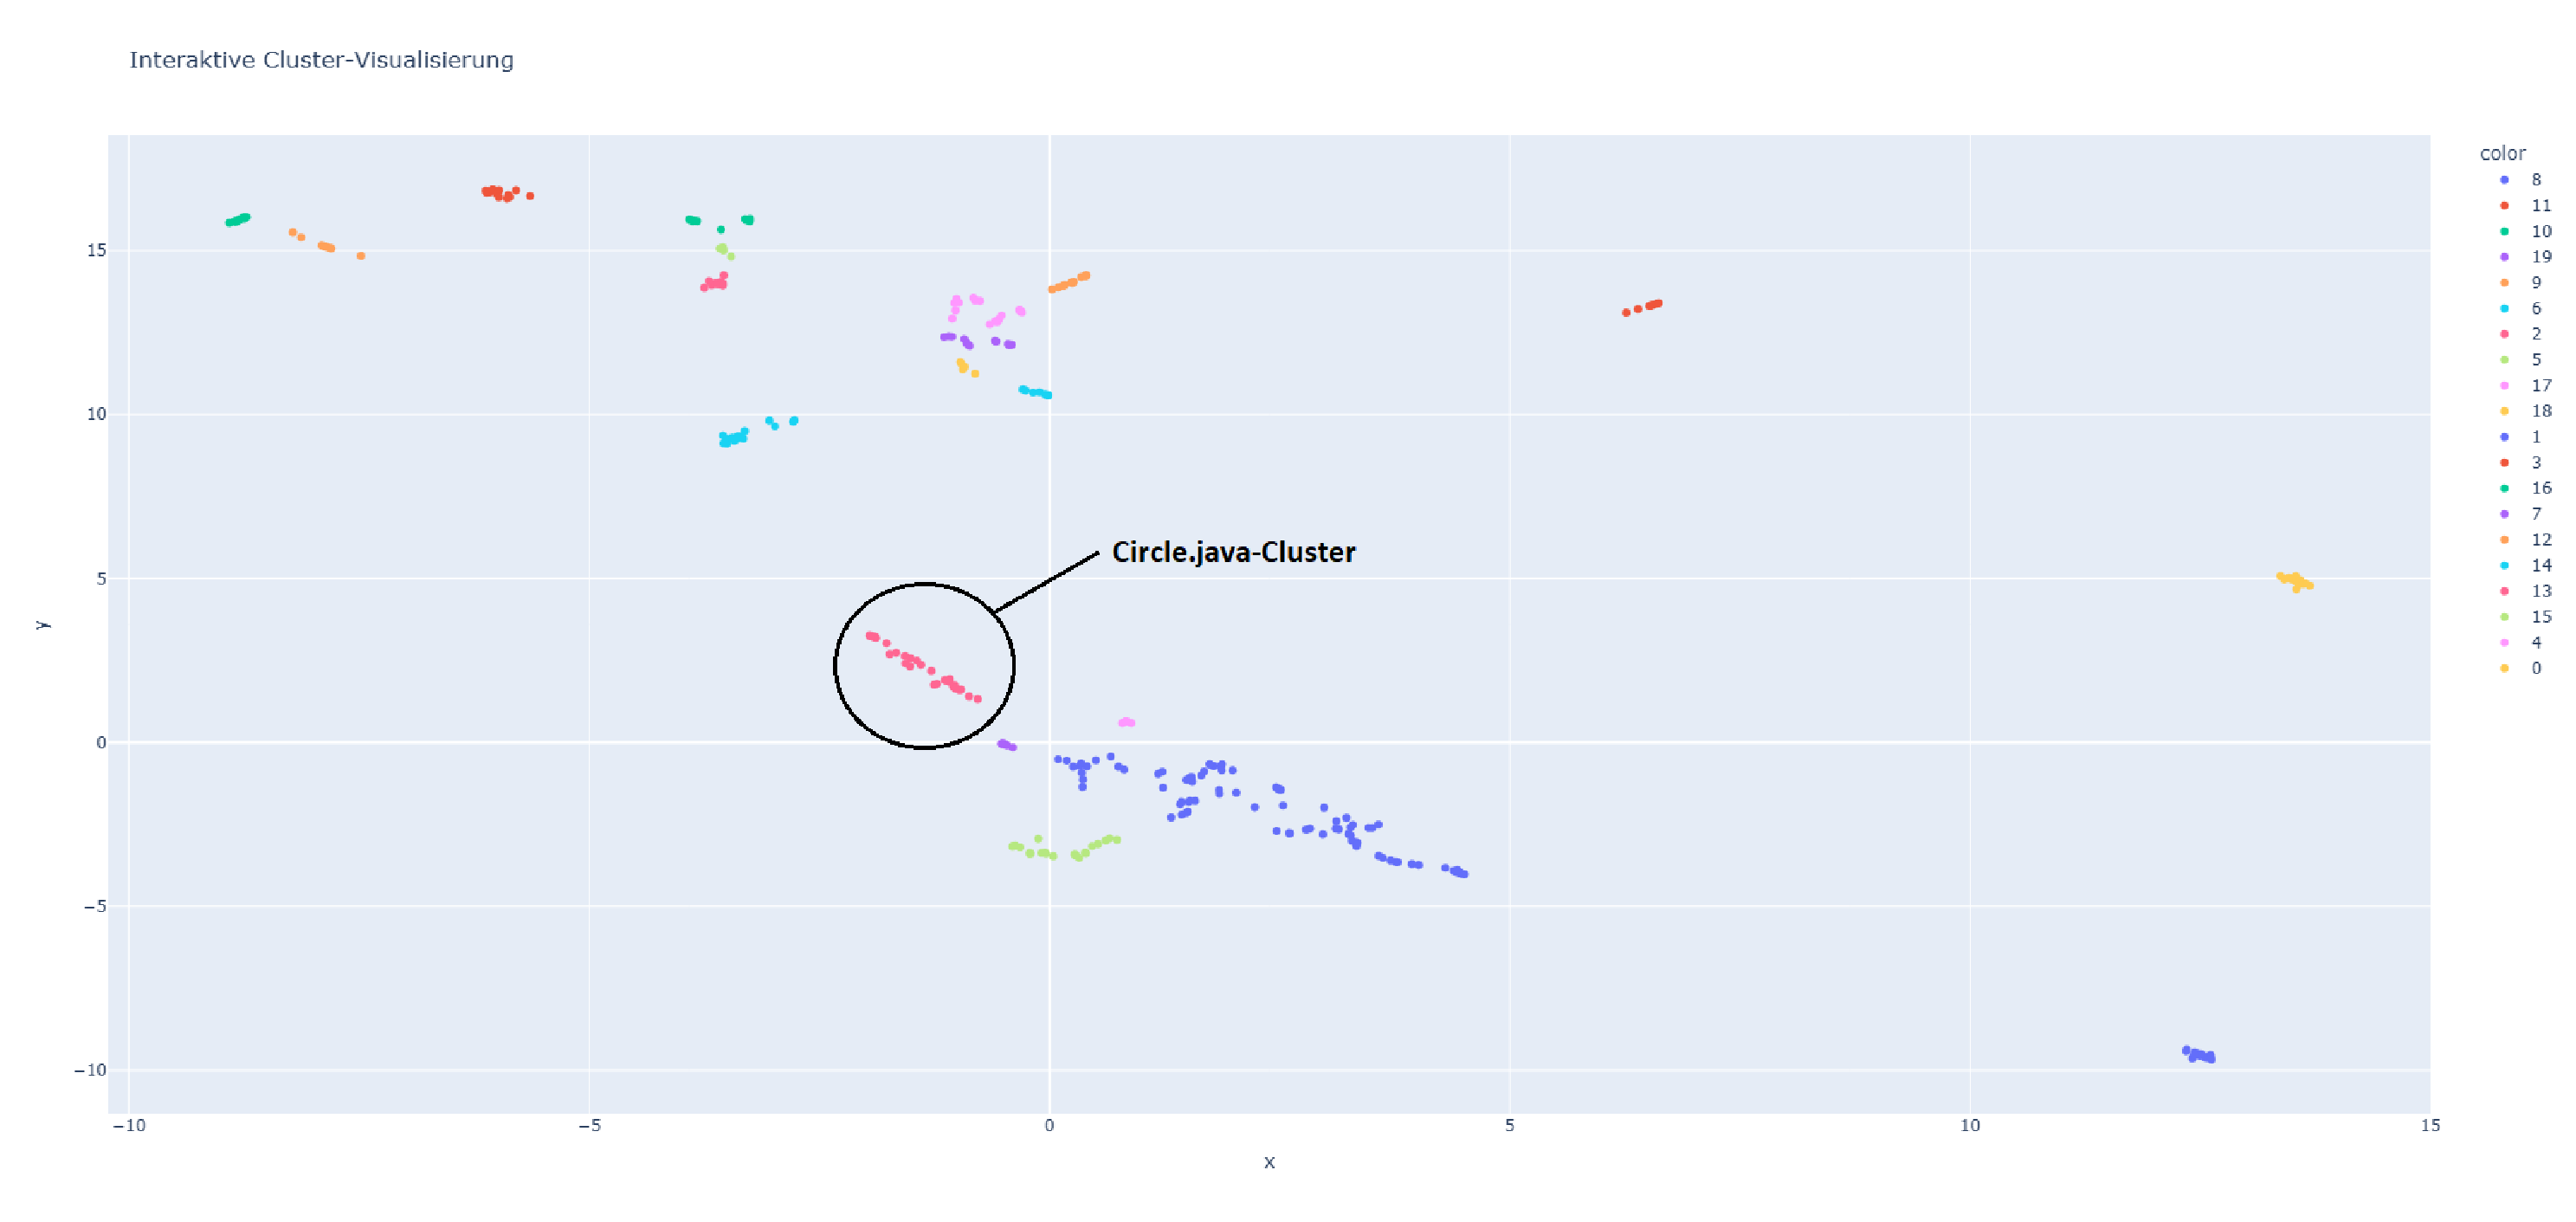
\includegraphics[width=1.0\textwidth]{images/Clusterung - 160 - gemischte Cluster.pdf}
	\caption{Zweiter Implementierungsabschnitt - Clustering-Diagramm einer Clusterung von 320 Java-Dateien. Der eingekreiste Cluster ist ein Circle.java-Cluster.}
	\label{abb:ZIa-C-160-gC}
\end{figure}

\begin{figure} %[hbtp]
	\centering
	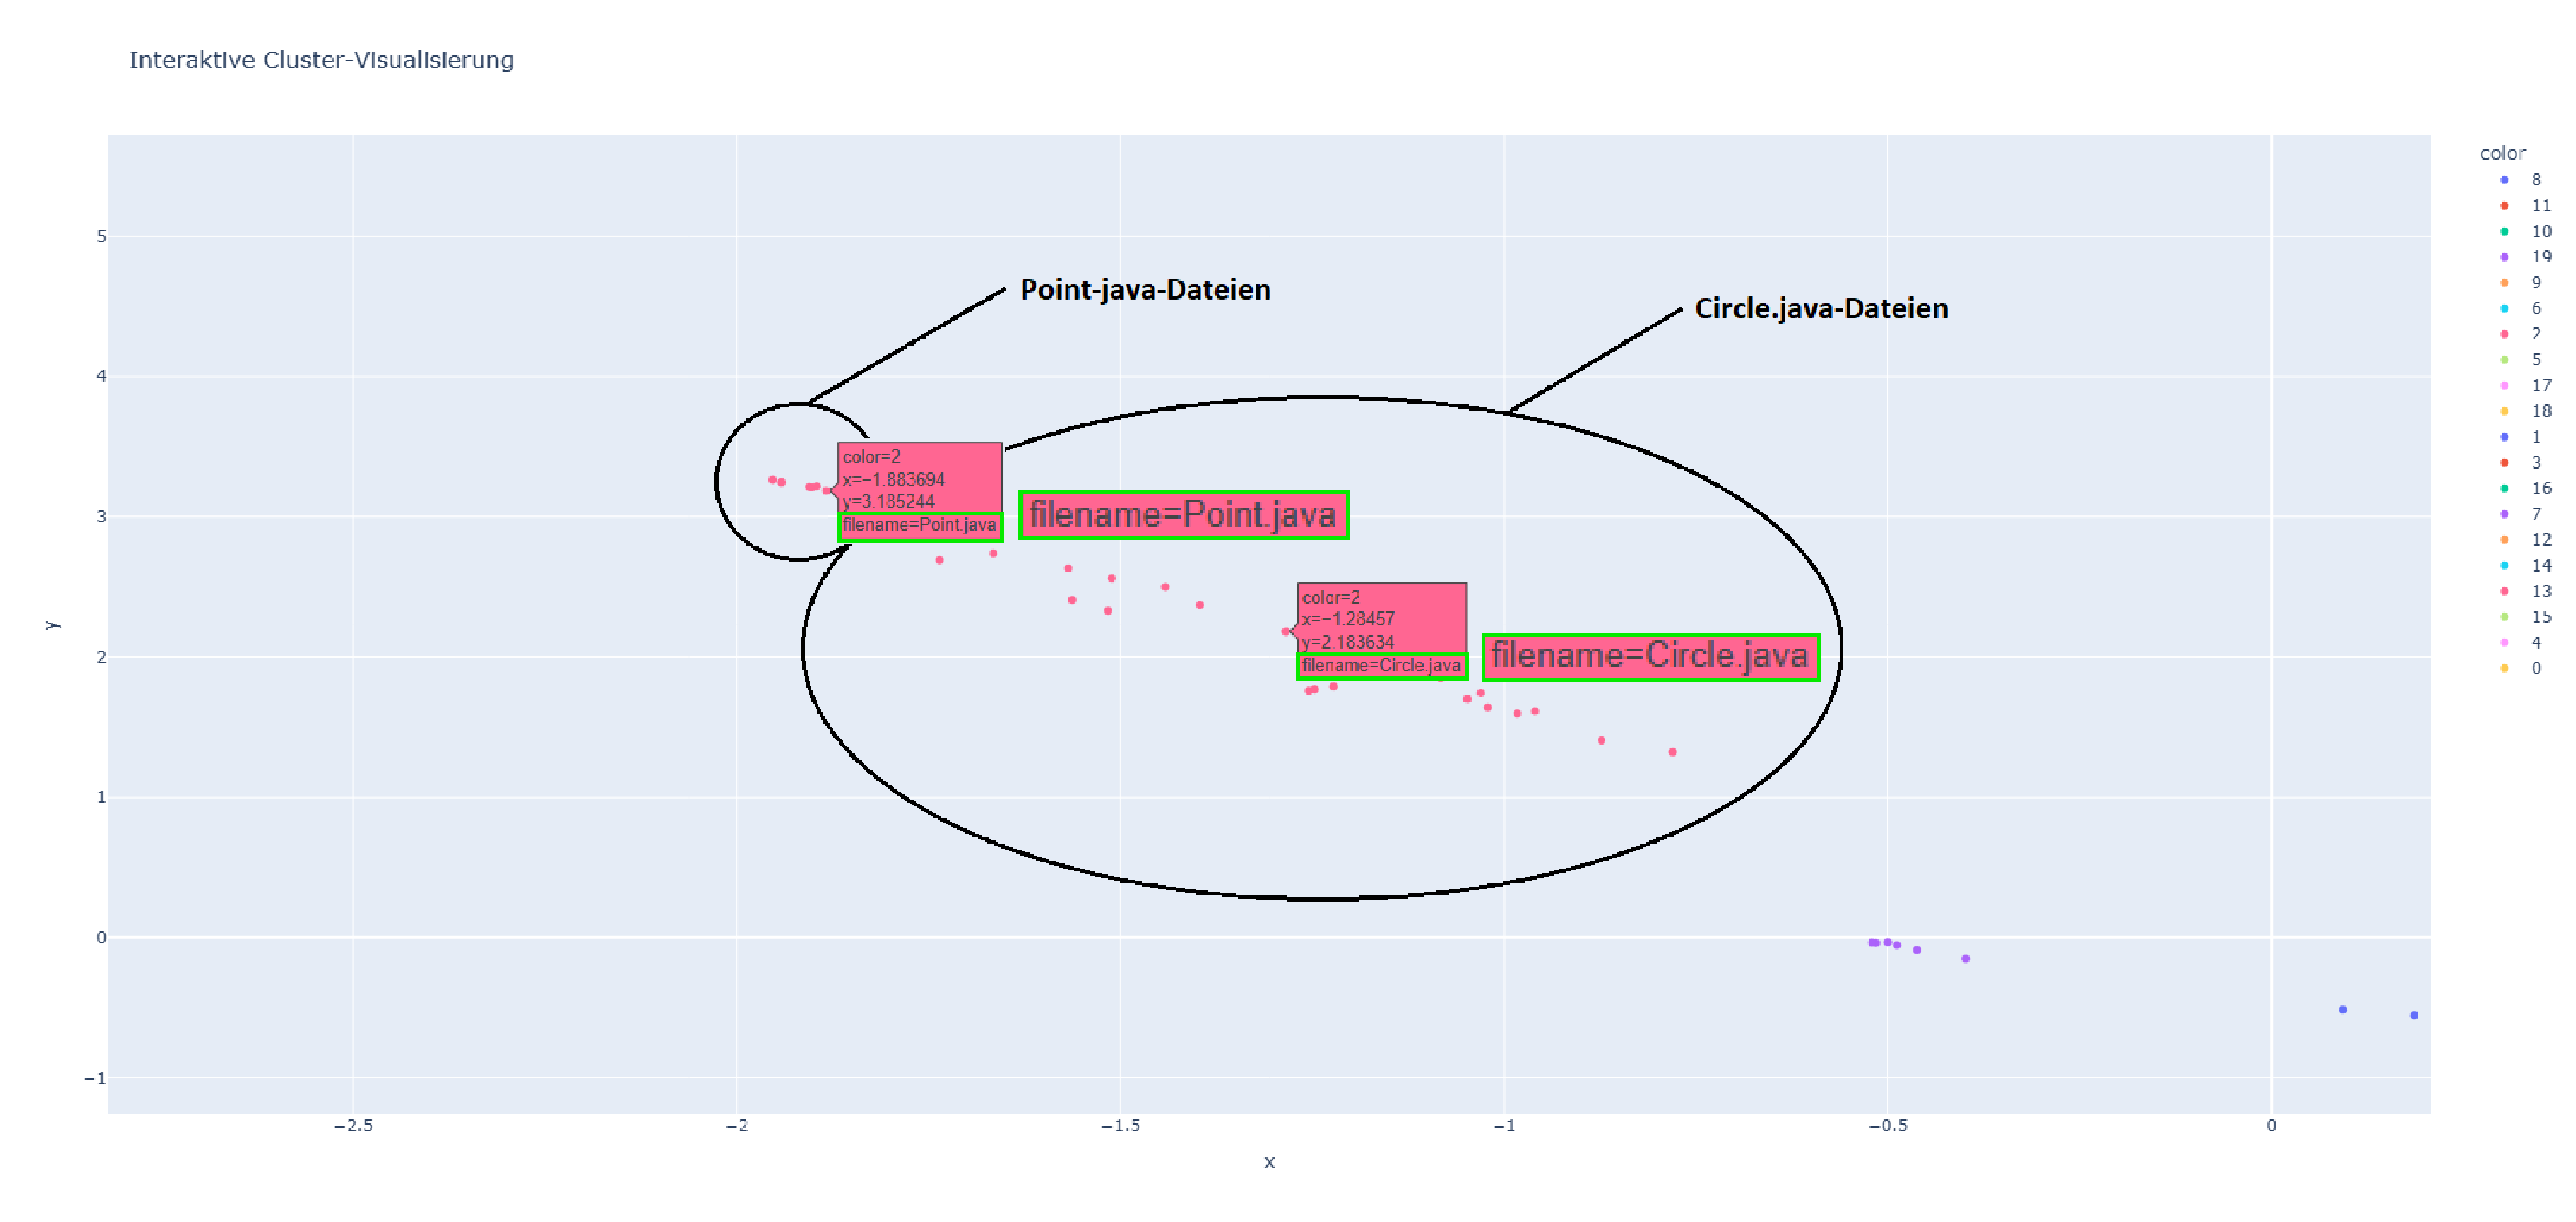
\includegraphics[width=1.0\textwidth]{images/Clusterung - 160 - gemischte Cluster - zoom.pdf}
	\caption{Zweiter Implementierungsabschnitt - Vergrößerter Circle.java-Cluster aus Abbildung \ref{abb:ZIa-C-160-gC}}
	\label{abb:ZIa-C-160-gC-z}
\end{figure}

\section{Ergebnisse - Finale Implementierung}
Anhand der finalen Implementierung kann nun ein realistisches Szenario getestet werden. Die Abbildungen \ref{abb:Miniprojekt-1-S.1} und \ref{abb:Miniprojekt-1-S.2} beschreibt eine beispielhafte Aufgabenstellung:

\begin{figure} %[hbtp]
	\centering
	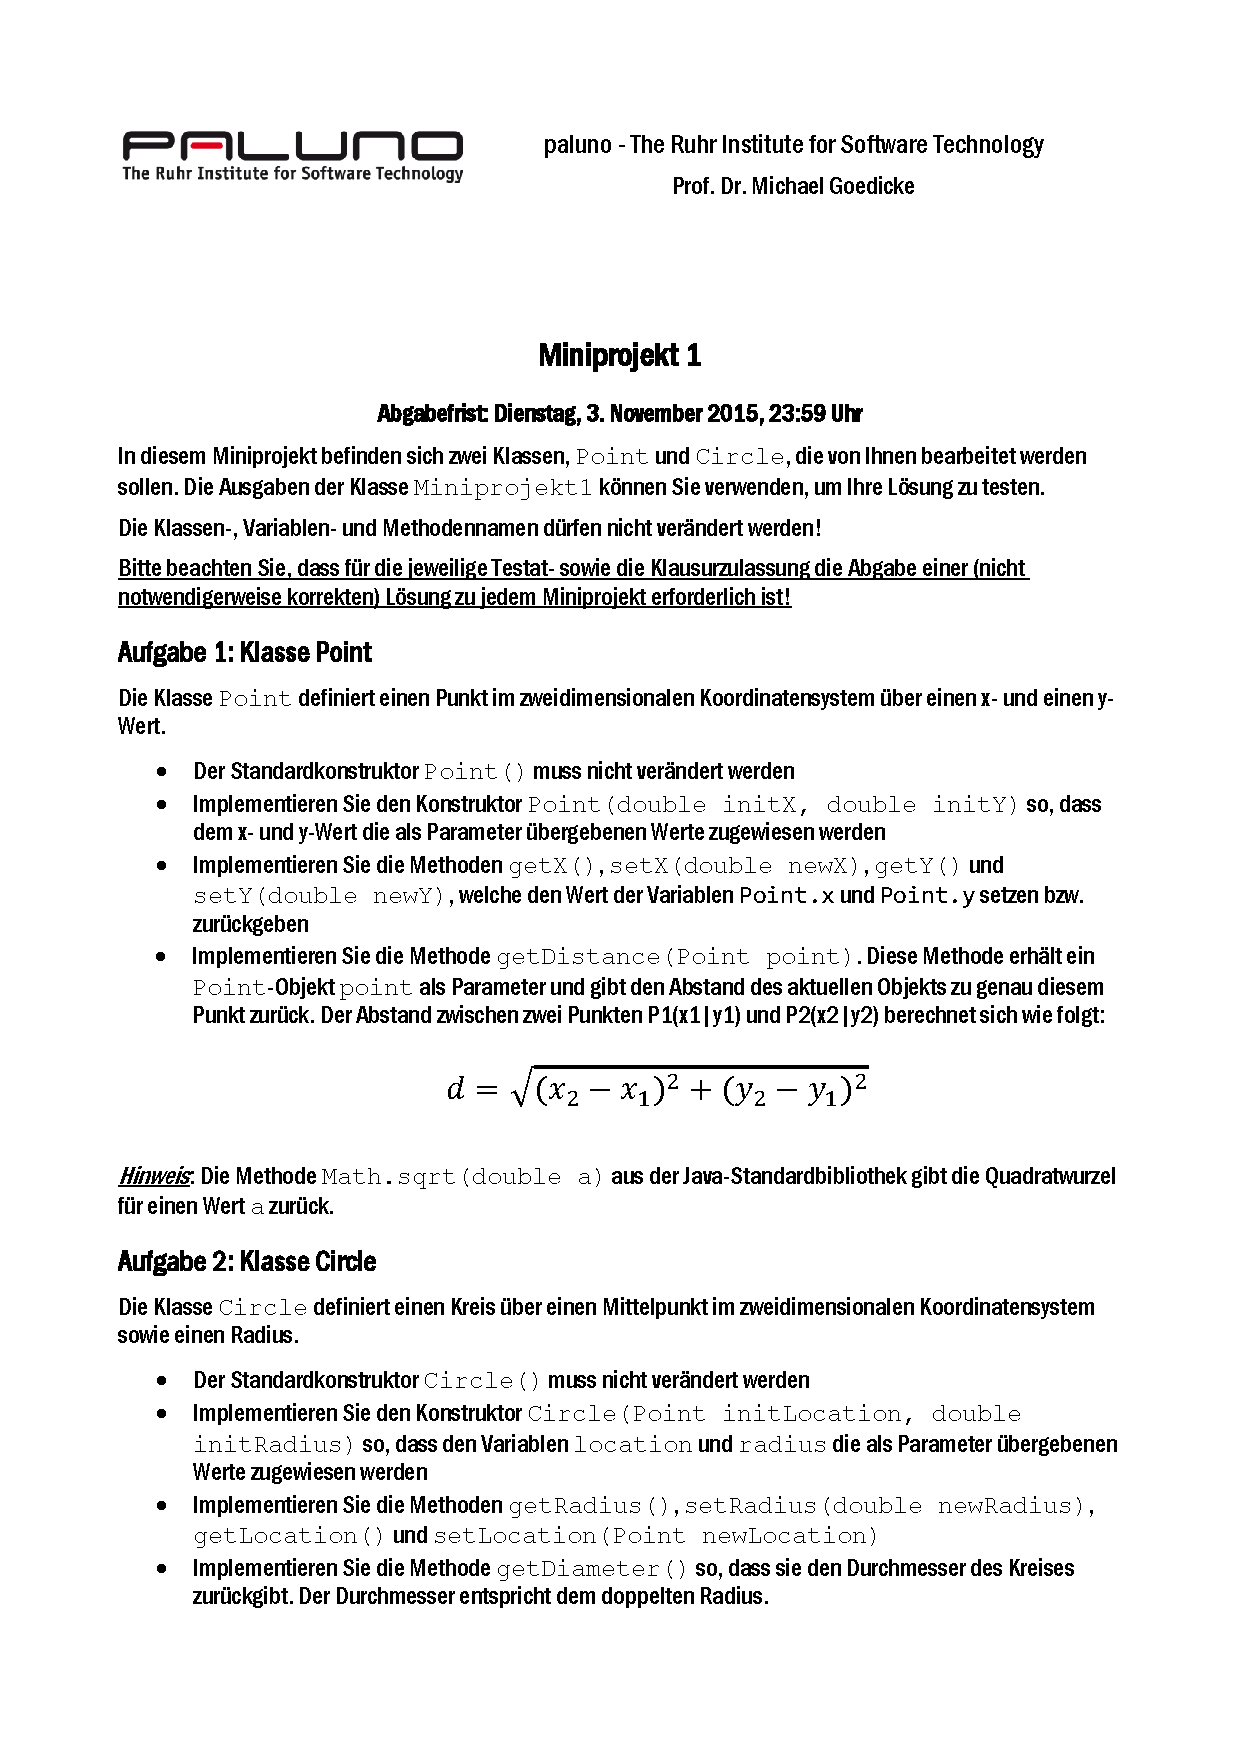
\includegraphics[width=1.0\textwidth]{images/Miniprojekt-1-S.1.pdf}
	\caption{Programmieraufagbe aus dem Jahr 2015 des paluno - The Ruhr Institute for Software Technology von Prof. Dr. Michael Goedicke, erste Seite}
	\label{abb:Miniprojekt-1-S.1}
\end{figure}

\begin{figure} %[hbtp]
	\centering
	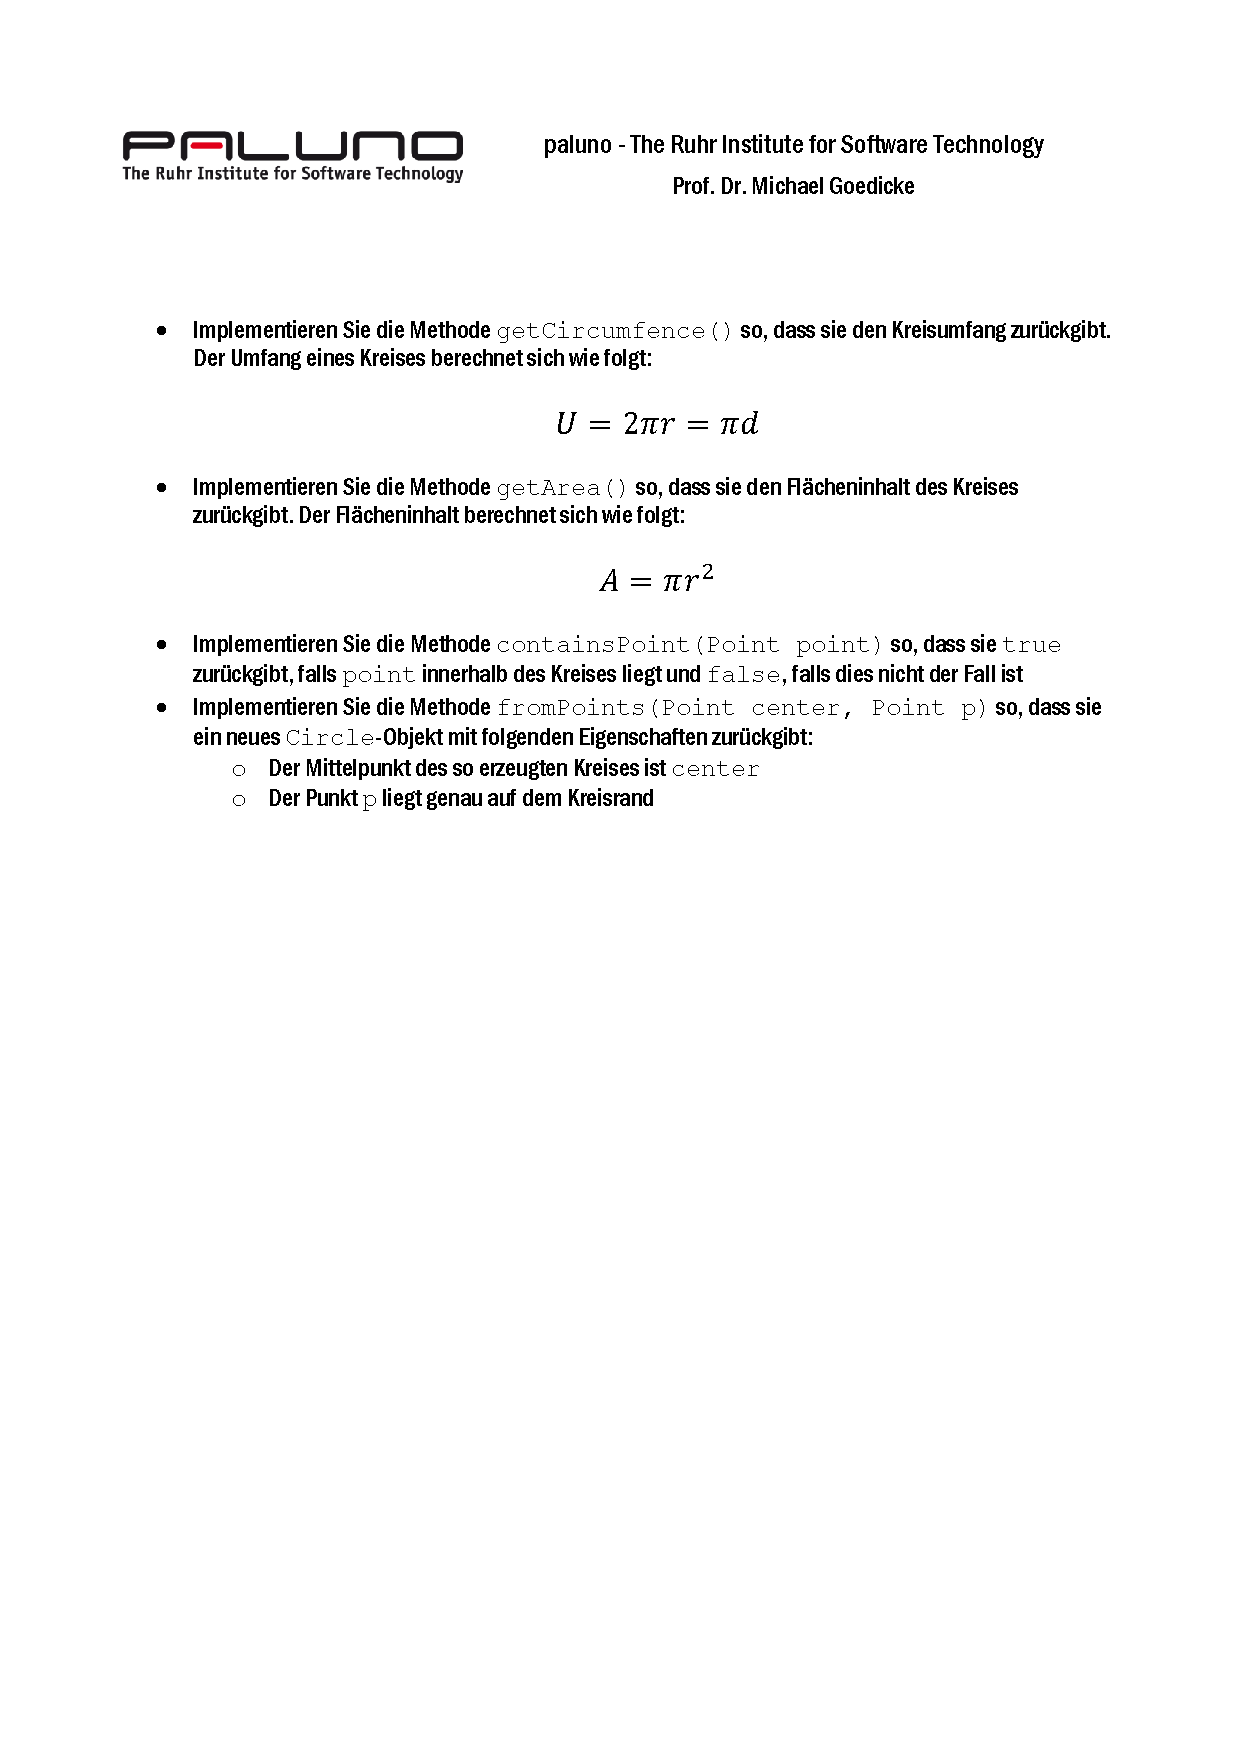
\includegraphics[width=1.0\textwidth]{images/Miniprojekt-1-S.2.pdf}
	\caption{Programmieraufagbe aus dem Jahr 2015 des paluno - The Ruhr Institute for Software Technology von Prof. Dr. Michael Goedicke, zweite Seite}
	\label{abb:Miniprojekt-1-S.2}
\end{figure}

Die zu bearbeitenden Java-Dateien waren Miniprojekt1, Point und Circle. Miniprojekt1-Dateien wurden ignoriert, da sie nicht bearbeitet werden sollten. Gefordert waren die Implementierung verschiedener Methoden der Point und Circle Klassen. Zunächst wurden die Einreichungen anhand der Experimentierungspipeline auf die beste Algorithmen-Kombination anhand Punktzahlenintervalle getestet. Sie wurden an das Notensystem angelehnt definiert (Note 1.0 bis 1.3 $\overset{\wedge}{=}$ Punktzahl $\geq$ 90, Note 1.7 bis 2.3 $\overset{\wedge}{=}$ Punktzahl $\geq$ 75, etc.), wobei perfekte Erebnisse (mit 100 Punkten bewertet) extra geclustert werden. Wenn die Dateimengen oder die Punktzahlenintervalle klein gewählt sind, treten dabei vermehrt Probleme der Algorithmen auf, die mit geringen Datenmengen nicht funktionieren. Deshalb wurde eine Menge von rund 1000 studentischen Einreichungen/Lösungen zum Testen verwendet (entspricht etwa 2000 einzelnen bzw. 1000 konkatenierten Dateien). Tabelle \ref{tab:FI-EI-EV-160-oPI} zeigt die Ergebnisse der Evaluationsmetriken ohne und Tabelle \ref{tab:FI-EI-EV-160-mPI} mit Punktzahlenintervalle. Trotz der Verfälschung in der zweiten Tabelle durch die Punktzahlenintervalle, stellte sich die Kombination UMAP mit k-Means als am besten heraus.

\setlength{\tabcolsep}{5.5pt}
\begin{table}[h]
\centering
\begin{tabular}{lcccc}
\hline
\textbf{Kombination} & \textbf{Silhouette} & \textbf{Calinski-Harabasz} & \textbf{Davies-Bouldin} & \textbf{Rang} \\
umap\_kmeans    & 0.479 & 2417.266 & 0.591 & 1 \\
pca\_kmeans     & 0.530 & 1872.106 & 0.495 & 2 \\
pca\_hdbscan    & 0.702 & 239.336  & 0.343 & 3 \\
tsne\_kmeans    & 0.373 & 1224.132 & 0.924 & 4 \\
umap\_hdbscan   & 0.110 & 845.411  & 0.473 & 5 \\
tsne\_hdbscan   & 0.530 & 40.382   & 1.750 & 6 \\
\hline
\end{tabular}
\caption{Finale Implementierung - Evaluationsergebnisse mit rund 1000 Dateien (ohne Punktzahlenintervalle).}
\label{tab:FI-EI-EV-160-oPI}
\end{table}

\setlength{\tabcolsep}{5.5pt}
\begin{table}[h]
\centering
\begin{tabular}{lcccc}
\hline
\textbf{Kombination} & \textbf{Silhouette} & \textbf{Calinski-Harabasz} & \textbf{Davies-Bouldin} & \textbf{Rang} \\
umap\_hdbscan   & -0.124 & 100.007 & 4.872 & 1 \\
umap\_kmeans    & -0.017 & 25.222  & 6.107 & 2 \\
pca\_kmeans     & -0.006 & 14.737  & 6.880 & 3 \\
pca\_hdbscan    &  0.067 & 17.322  & 9.449 & 4 \\
tsne\_kmeans    & -0.033 & 11.893  & 9.075 & 5 \\
tsne\_hdbscan   & -0.494 & 2.994   & 20.513 & 6 \\
\hline
\end{tabular}
\caption{Finale Implementierung - Evaluationsergebnisse mit rund 1000 Dateien (mit Punktzahlenintervalle).}
\label{tab:FI-EI-EV-160-mPI}
\end{table}

Als nächstes wurde die Pipeline verwendet, um die Clusterungen zu visualisieren. Abbildung \ref{abb:C-1000} zeigt das entstandene Diagramm, wobei die unterschiedlichen Farben und Überlappung der Cluster durch die Punktzahlenintervalle zustande kamen und damit visuell weniger wertvoll sind. Aus diesem Grund wurde auf die erstellte CSV-Datei aus dem cluster\_report zurückgegriffen. Nun galt es zu überprüfen ob für die Cluster jeweils ein identisches Feedback ausreicht. Dafür wurden aus jedem Cluster zwei Kandidaten ausgesucht und nach Fehlerarten gesucht, welche das jeweilige Feedback bestimmen würden. Die Tabellen \ref{tab:A-d-CD}, \ref{tab:A-d-PD} und \ref{tab:Abk} zeigen die Ergebnisse. Die ersten beiden Tabellen stehen dabei für die Auswertung der Circle- und Point-Dateien und die letzte für die verwendeten Abkürzungen. Sie sind sortiert nach Punktzahlenintervalle (Sc.-B.), Cluster, Aufgabenart (C1-C10, P1-P6), Einreichungen (aus Platzgründen zu Punktzahl und "P" abgekürzt, z. B. "53 P") und ob die Antworten gleich oder ungleich waren. Die Ergebnisse zeigen, dass die Zahl der gleichen Antworten nach steigenden Punktzahlenintervallen entsprechend mitwächst. Identisches Feedback ist erst bei einer 100-prozentigen Übereinstimmung der Antworten sinnvoll. Hier wäre es also nur im Bereich 60-74 und 90-99 angebracht identisches Feedback zu generieren. Um mehr gewährleisten zu können, würde womöglich eine weitere Spezialisierung der Punktzahlenintervalle als Idee nahe erscheinen, jedoch wurden bei einer identischen Punktzahl (53 und 53 in Sc.-B. 50-59) nur ungleiche Antworten gegeben. Es ist also eine Verallgemeinerung der Antwortarten oder des Feedbacks notwendig. Weiterhin könnten Tests mit verschiedenen Algorithmen-Kombinationen für präzisere Ergebnisse sorgen.

\begin{figure} %[hbtp]
	\centering
	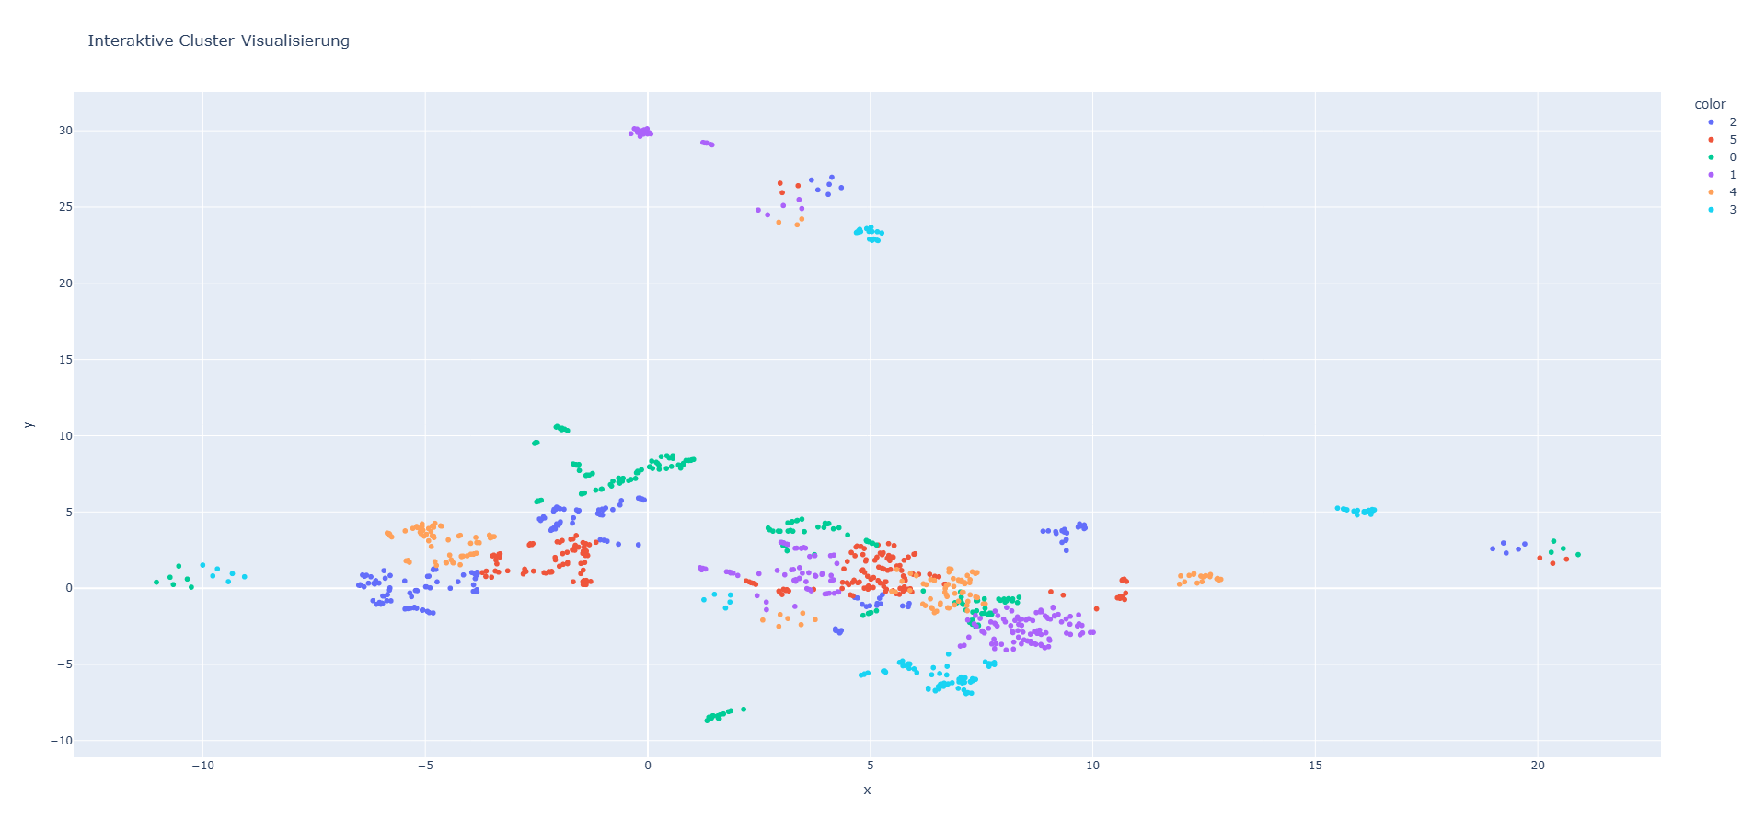
\includegraphics[width=1.0\textwidth]{images/Clusterung - 1000.pdf}
	\caption{Finale Implementierung - Clusterung von rund 1000 Dateien. Pro Farbe wird weiter durch Punktzahlenintervalle unterschieden}
	\label{abb:C-1000}
\end{figure}

\begin{table}[h]
    \centering
    \begin{tabular}{|l|l|l|l|l|l|l|l|l|l|l|l|l|}
    \hline
        Sc.-B. 0-49 & C1 & C2 & C3 & C4 & C5 & C6 & C7 & C8 & C9 & C10 & gl. & ungl. \\ \hline
        Cluster 0: & ~ & ~ & ~ & ~ & ~ & ~ & ~ & ~ & ~ & ~ & ~ & ~ \\ \hline
             0 P & A1 & A1 & A1 & A1 & A1 & A1 & A1 & A1 & A2 & A3 & ~ & ~ \\ \hline
             49 P & A4 & A5 & A4 & A6 & A4 & A5 & A9 & A5 & A7 & A4 & ~ & ~ \\ \hline
        ~ & 0 & 0 & 0 & 0 & 0 & 0 & 0 & 0 & 0 & 0 & 0 & 10 \\ \hline
        Sc.-B. 50-59 & ~ & ~ & ~ & ~ & ~ & ~ & ~ & ~ & ~ & ~ & ~ & ~ \\ \hline
        Cluster 3: & ~ & ~ & ~ & ~ & ~ & ~ & ~ & ~ & ~ & ~ & ~ & ~ \\ \hline
          53 P & A4 & A5 & A4 & A6 & A4 & A5 & A9 & A5 & A7 & A4 & ~ & ~ \\ \hline
          53 P & A1 & A1 & A1 & A1 & A1 & A1 & A1 & A1 & A1 & A8 & ~ & ~ \\ \hline
        ~ & 0 & 0 & 0 & 0 & 0 & 0 & 0 & 0 & 0 & 0 & 0 & 10 \\ \hline
        Sc.-B.  60-74 & ~ & ~ & ~ & ~ & ~ & ~ & ~ & ~ & ~ & ~ & ~ & ~ \\ \hline
        Cluster 1: & ~ & ~ & ~ & ~ & ~ & ~ & ~ & ~ & ~ & ~ & ~ & ~ \\ \hline
          66 P & A1 & A1 & A1 & A6 & A1 & A5 & A9 & A5 & A7 & A4 & ~ & ~ \\ \hline
          70 P & A1 & A1 & A1 & A1 & A1 & A5 & A9 & A5 & A7 & A4 & ~ & ~ \\ \hline
        ~ & 1 & 1 & 1 & 0 & 1 & 1 & 1 & 1 & 1 & 1 & 9 & 1 \\ \hline
        Sc.-B. 75-90 & ~ & ~ & ~ & ~ & ~ & ~ & ~ & ~ & ~ & ~ & ~ & ~ \\ \hline
        Cluster 0: & ~ & ~ & ~ & ~ & ~ & ~ & ~ & ~ & ~ & ~ & ~ & ~ \\ \hline
          75 P & A1 & A1 & A1 & A1 & A1 & A10 & A10 & A10 & A11 & A4 & ~ & ~ \\ \hline
          87 P & A1 & A1 & A1 & A1 & A1 & A1 & A1 & A1 & A7 & A4 & ~ & ~ \\ \hline
        ~ & 1 & 1 & 1 & 1 & 1 & 0 & 0 & 0 & 0 & 1 & 6 & 4 \\ \hline
        Sc.-B. 90-99 & ~ & ~ & ~ & ~ & ~ & ~ & ~ & ~ & ~ & ~ & ~ & ~ \\ \hline
        Cluster 1: & ~ & ~ & ~ & ~ & ~ & ~ & ~ & ~ & ~ & ~ & ~ & ~ \\ \hline
          92 P & A1 & A1 & A1 & A1 & A1 & A1 & A1 & A1 & A1 & A4 & ~ & ~ \\ \hline
          96 P & A1 & A1 & A1 & A1 & A1 & A1 & A12 & A1 & A13 & A1 & ~ & ~ \\ \hline
    \end{tabular}
	\caption{Finale Implementierung - Auswertung der Circle-Dateien}
\label{tab:A-d-CD}
\end{table}

\begin{table}[h]
    \centering
    \begin{tabular}{|l|l|l|l|l|l|l|l|l|}
    \hline
        Sc.-B. 0-49 & P1 & P2 & P3 & P4 & P5 & P6 & gl. & ungl. \\ \hline
        Cluster 0: & ~ & ~ & ~ & ~ & ~ & ~ & ~ & ~ \\ \hline
             0 P & A1 & A4 & A4 & A4 & A4 & A4 & ~ & ~ \\ \hline
             49 P & A15 & A1 & A1 & A1 & A1 & A1 & ~ & ~ \\ \hline
        ~ & 0 & 0 & 0 & 0 & 0 & 0 & 0 & 6 \\ \hline
        Sc.-B. 50-59 & ~ & ~ & ~ & ~ & ~ & ~ & ~ & ~ \\ \hline
        Cluster 3: & ~ & ~ & ~ & ~ & ~ & ~ & ~ & ~ \\ \hline
          53 P & A1 & A1 & A1 & A1 & A1 & A1 & ~ & ~ \\ \hline
          53 P & A4 & A5 & A4 & A5 & A4 & A5 & ~ & ~ \\ \hline
        ~ & 0 & 0 & 0 & 0 & 0 & 0 & 0 & 6 \\ \hline
        Sc.-B.  60-74 & ~ & ~ & ~ & ~ & ~ & ~ & ~ & ~ \\ \hline
        Cluster 1: & ~ & ~ & ~ & ~ & ~ & ~ & ~ & ~ \\ \hline
          66 P & A1 & A1 & A1 & A1 & A1 & A14 & ~ & ~ \\ \hline
          70 P & A1 & A1 & A1 & A1 & A1 & A14 & ~ & ~ \\ \hline
        ~ & 1 & 1 & 1 & 1 & 1 & 1 & 6 & 0 \\ \hline
        Sc.-B. 75-90 & ~ & ~ & ~ & ~ & ~ & ~ & ~ & ~ \\ \hline
        Cluster 0: & ~ & ~ & ~ & ~ & ~ & ~ & ~ & ~ \\ \hline
          75 P & A1 & A1 & A1 & A1 & A1 & A10 & ~ & ~ \\ \hline
          87 P & A1 & A1 & A1 & A1 & A1 & A1 & ~ & ~ \\ \hline
        ~ & 1 & 1 & 1 & 1 & 1 & 0 & 5 & 1 \\ \hline
        Sc.-B. 90-99 & ~ & ~ & ~ & ~ & ~ & ~ & ~ & ~ \\ \hline
        Cluster 1: & ~ & ~ & ~ & ~ & ~ & ~ & ~ & ~ \\ \hline
          92 P & A1 & A1 & A1 & A1 & A1 & A1 & ~ & ~ \\ \hline
          96 P & A1 & A1 & A1 & A1 & A1 & A1 & ~ & ~ \\ \hline
        ~ & 1 & 1 & 1 & 1 & 1 & 1 & 6 & 0 \\ \hline
    \end{tabular}
	\caption{Finale Implementierung - Auswertung der Point-Dateien}
\label{tab:A-d-PD}
\end{table}

\begin{table}[h]
    \centering
    \begin{tabular}{|l|l|}
    \hline
        Aufgaben: & Abkürzungen: \\ \hline
        Circle(Point initLocation, double initRadius) & C1 \\ \hline
        getRadius() & C2 \\ \hline
        setRadius(double newRadius) & C3 \\ \hline
        getLocation() & C4 \\ \hline
        setLocation(Point newLocation) & C5 \\ \hline
        getDiameter() & C6 \\ \hline
        getCircumfence() & C7 \\ \hline
        getArea() & C8 \\ \hline
        containsPoint(Point point) & C9 \\ \hline
        fromPoints(Point center, Point p) & C10 \\ \hline
        ~ & ~ \\ \hline
        Point(double initX, double initY) & P1 \\ \hline
        getX() & P2 \\ \hline
        setX(double newX) & P3 \\ \hline
        getY() & P4 \\ \hline
        setY(double newY) & P5 \\ \hline
        getDistance(Point point) & P6 \\ \hline
        ~ & ~ \\ \hline
        Antworten: & Abkürzungen: \\ \hline
        richtig & A1 \\ \hline
        falsche Einrückung im else-Fall & A2 \\ \hline
        Point hat keine Methode getDiameter() & A3 \\ \hline
        fehlt & A4 \\ \hline
        return -1.0 & A5 \\ \hline
        return new Point() & A6 \\ \hline
        return false & A7 \\ \hline
        center = circle.getLocation(); & A8 \\ \hline
        return Math.PI & A9 \\ \hline
        return 0.0 & A10 \\ \hline
        Quadrat- statt Kreisüberprüfung & A11 \\ \hline
        return Math.PI * getCircumference() & A12 \\ \hline
        if(point.getDistance(location)> getRadius()) & A13 \\ \hline
        Es fehlt eine Klammer bei Math.sqrt() & A14 \\ \hline
        initY = y & A15 \\ \hline
    \end{tabular}
	\caption{Finale Implementierung - Antwortabkürzungen}
\label{tab:Abk}
\end{table}
\chapter{Zusammenfassung und Ausblick}

In diesem Kapitel soll die Arbeit noch einmal kurz zusammengefasst werden. Insbesondere sollen die wesentlichen Ergebnisse Ihrer Arbeit herausgehoben werden. Erfahrungen, die z.B. Benutzer mit der Mensch-Maschine-Schnittstelle gemacht haben oder Ergebnisse von Leistungsmessungen sollen an dieser Stelle präsentiert werden. Sie können in diesem Kapitel auch die Ergebnisse oder das Arbeitsumfeld Ihrer Arbeit kritisch bewerten. Wünschenswerte Erweiterungen sollen als Hinweise auf weiterführende Arbeiten erwähnt werden.

\chapter{Anhang}

\begin{lstlisting}[language=Python, caption={Pipeline}, label={prco:Pipel}]
import os
import yaml
import warnings
import numpy as np
from utils.data_loader import DataLoader
from embeddings.embedding_model import EmbeddingModel
from dimReducer.dimension_reducer import DimensionReducer
from clustering.clustering_engine import ClusteringEngine
from utils.score_binning import ScoreBinner
from visualization.advanced_interactive_plot import AdvancedInteractivePlot
from evaluation.evaluation_metrics import EvaluationMetrics
from reporting.report_generator import ReportGenerator

# load config
def load_config(path="config.yaml"):
    with open(path, "r") as file:
        return yaml.safe_load(file)

def run_pipeline():
    config = load_config()

    # ignore warnings
    warnings.filterwarnings("ignore", category=FutureWarning)
    warnings.filterwarnings("ignore", category=UserWarning)

    # dynamically determine path
    base_path = os.path.dirname(os.path.abspath(__file__))
    input_path = os.path.join(base_path, config['data']['input_path'])

    # load data
    loader = DataLoader(config['data']['files_to_look_for'],
                        input_path,
                        config['data']['exclude_files'],
                        config['data']['exclude_folders'])
    code_snippets = loader.load_code_files(concat=True)

    # score bins
    scores = loader.get_scores()
    binned_scores = ScoreBinner.bin_scores(scores,
                                config['data']['score_bins'])
                                unique_bins = sorted(set(binned_scores))

    # Embedding object
    model = EmbeddingModel(config['embedding']['model'])
    cache_path = "cached_embeddings.npy"

    # save all info resulting in the loop to display it in one plot later
    all_embeddings, all_labels, all_filenames,
        all_parent_dirs, all_score_bins = [], [], [], [], []

    # filter solutions by score bin and prepare data for clustering
    for score_bin in unique_bins:
        print(f"\n==== Processing score_bin: {score_bin} ====")
        indices =
            [i for i, b in enumerate(binned_scores) if b == score_bin]

        if len(indices) < 4:
            continue    # Not enough solutions in score_bin

        snippets_bin = [code_snippets[i] for i in indices]
        filenames_bin = [loader.get_filenames()[i] for i in indices]
        parent_dirs_bin = [loader.get_parent_dirs()[i] for i in indices]

        # Embedding
        if os.path.exists(cache_path):
            embeddings_cache = np.load(cache_path)
            if len(embeddings_cache) >= len(snippets_bin):
                embeddings = embeddings_cache[:len(snippets_bin)]
            else:
                embeddings = np.array(
                    [model.get_embedding(code) for code in snippets_bin])
                np.save(cache_path, embeddings)
        else:
            embeddings = np.array(
                [model.get_embedding(code) for code in snippets_bin])
            np.save(cache_path, embeddings)

        # Dimension reduction
        reducer = DimensionReducer(config['dim_reduction']['algorithm'],
                                   config['dim_reduction']['params'])
        reduced_embeddings = reducer.reduce(embeddings)

        # Clustering
        clusterer = ClusteringEngine(config['clustering']['algorithm'],
                                     config['clustering']['params'])
        labels = clusterer.cluster(reduced_embeddings)

        # Evaluation
        results = EvaluationMetrics.evaluate(reduced_embeddings, labels)
        print("Evaluation results:", results)

        # Save info for interactive plot
        all_embeddings.extend(reduced_embeddings)
        all_labels.extend(labels)
        all_filenames.extend(filenames_bin)
        all_parent_dirs.extend(parent_dirs_bin)
        all_score_bins.extend([score_bin] * len(labels))

    # Interactive plot
    AdvancedInteractivePlot.plot(all_embeddings,
                                 all_labels,
                                 all_filenames,
                                 all_parent_dirs,
                                 all_score_bins)
    # Reporting
    ReportGenerator.generate_report(all_filenames,
                                    all_parent_dirs,
                                    all_labels,
                                    all_score_bins,
                                    config['data']['output_path'])
    print(f"Report saved to {config['data']['output_path']}")

if __name__ == "__main__":
    run_pipeline()
\end{lstlisting}


\begin{lstlisting}[language=Python, caption={Konfigurationsdatei}, label={prco:Konfigurationsdatei}]
embedding:
  model: "microsoft/codebert-base"  # embedding model for code snippets

dim_reduction:
# --- umap ---
  algorithm: "umap"
  params:
    n_components: 2
    n_neighbors: 15
    min_dist: 0.1
    metric: "euclidean"
    random_state: 42
    spread: 1.0
    learning_rate: 1.0
    init: "spectral"
# # --- pca ---
#   algorithm: "pca"
#   params:
#     n_components: 2
#     svd_solver: "auto"
#     random_state: 42
# # --- t-sne ---
#   algorithm: "tsne"
#   params:
#     n_components: 2
#     perplexity: 30.0
#     learning_rate: 200.0
#     n_iter: 1000
#     metric: "euclidean"
#     random_state: 42
#     init: "random"
#     early_exaggeration: 12.0
#     angle: 0.5
#     verbose: 0

clustering:
# --- hdbscan ---
  # algorithm: "hdbscan"
  # params:
  #   min_cluster_size: 2
  #   min_samples: 1
  #   cluster_selection_epsilon: 0.5
  #   metric: "euclidean"
  #   cluster_selection_algorithm: "eom"
  #   alpha: 1.0
  #   allow_single_cluster: false
# --- k-means ---
  algorithm: "kmeans"
  params:
    n_clusters: 5
    init: "k-means++"
    n_init: 10
    max_iter: 300
    random_state: 42

data:
  files_to_look_for: ".java"
  exclude_files: ["Miniprojekt1.java"]
  exclude_folders: ["100 Punkte"]
  input_path: "C:/Users/grego/Desktop/Loesungen/000TestingMedium000"
  output_path: "z_Output"
  score_bins:
  [[100, 100], [95, 99], [90, 94], [50, 89], [0, 49]]
\end{lstlisting}


\begin{lstlisting}[language=Python, caption={\texttt{data\_loader.py}}, label={prco:data-loader}]
import os

class DataLoader:
    def __init__(self, file_name, data_path, exclude_files=None, 
    exclude_folders=None):
        self.data_path = data_path
        self.file_name = file_name
        self.filenames = []
        self.exclude_files = exclude_files if exclude_files else []
        self.exclude_folders = exclude_folders if exclude_folders else []
        self.parent_dirs = []

    def load_code_files(self, concat=False):
        results = []
        # walk through all subdirectories
        for root, dirs, files in os.walk(self.data_path):
            if any(excl in root for excl in self.exclude_folders):
                continue    # skip excluded folders

            desired_files = [f for f in files 
                if f.endswith(self.file_name) and 
                f not in self.exclude_files]
            if not desired_files:
                continue    # find matching files and skip excluded files

            solution_code = ""
            for file in desired_files:
                file_path = os.path.join(root, file)
                with open(file_path, "r", encoding="utf-8", 
                errors="ignore") as f:
                    content = f.read()
                    if concat: # concatenate file contents
                        solution_code += content + "\n"
                    else:
                        results.append(content)

                self.filenames.append(file)

            # extract folder names (parent directory and score folder)
            score_dir = os.path.basename(root)
            student_id = os.path.basename(os.path.dirname(root))
            self.parent_dirs.append((student_id, score_dir))

            if concat:
                results.append(solution_code)
        return results
    
    def get_scores(self):
        scores = []
        for parent_tuple in self.parent_dirs:
            score_dir = parent_tuple[1]
            try:
                score = int(''.join(filter(str.isdigit, 
                    score_dir.split(' Punkte')[0].split()[-1])))
            except ValueError:
                score = -1
            scores.append(score)
        return scores

    def get_filenames(self):
        return self.filenames
    def get_parent_dirs(self):
        return self.parent_dirs
\end{lstlisting}


\begin{lstlisting}[language=Python, caption={\texttt{score\_binning.py}}, label={prco:score-binning}]
class ScoreBinner:
    @staticmethod
    def bin_scores(scores, bins):
        binned_labels = []
        for score in scores:
            binned_label = None
            for low, high in bins:
                if low <= score <= high:
                    binned_label = f"{low}-{high}"  # label string for bin
                    break
            if binned_label is None:  # if no bin matched the score
                binned_label = "Unassigned"  # assign 'Unassigned' label
            binned_labels.append(binned_label)
        return binned_labels
\end{lstlisting}

\begin{lstlisting}[language=Python, caption={\texttt{embedding\_model.py}}, label={prco:embedding-model}]
from transformers import AutoTokenizer, AutoModel
import torch

class EmbeddingModel:
    def __init__(self, model_name):
        self.tokenizer = AutoTokenizer.from_pretrained(model_name)
        self.model = AutoModel.from_pretrained(model_name)

    def get_embedding(self, code_snippet):
        tokens = self.tokenizer(code_snippet, return_tensors="pt", 
                                truncation=True, padding=True)
        with torch.no_grad():
            outputs = self.model(**tokens)
        return outputs.last_hidden_state.mean(dim=1).squeeze().numpy()
\end{lstlisting}

\begin{lstlisting}[language=Python, caption={\texttt{dimension\_reducer.py}}, label={prco:dimension-reducer}]
class DimensionReducer:
    def __init__(self, algorithm="umap", params=None):
        self.algorithm = algorithm
        self.params = params if params is not None else {}

    def reduce(self, embeddings):
        if self.algorithm == "pca":
            from sklearn.decomposition import PCA
            model = PCA(**self.params)
        elif self.algorithm == "tsne":
            from sklearn.manifold import TSNE
            model = TSNE(**self.params)
        elif self.algorithm == "umap":
            import umap
            model = umap.UMAP(**self.params)
        else:
            raise ValueError(f"Unsupported algorithm: {self.algorithm}")

        reduced_embeddings = model.fit_transform(embeddings)
        return reduced_embeddings
\end{lstlisting}

\begin{lstlisting}[language=Python, caption={\texttt{clustering\_engine.py}}, label={prco:clustering-engine}]
class ClusteringEngine:
    def __init__(self, algorithm="hdbscan", params=None):
        self.algorithm = algorithm
        self.params = params if params is not None else {}

    def cluster(self, reduced_embeddings):
        if self.algorithm == "kmeans":
            from sklearn.cluster import KMeans
            model = KMeans(**self.params)
        elif self.algorithm == "hdbscan":
            import hdbscan
            model = hdbscan.HDBSCAN(**self.params)
        else:
            raise ValueError(f"Unsupported algorithm: {self.algorithm}")

        labels = model.fit_predict(reduced_embeddings)
        return labels
\end{lstlisting}

\begin{lstlisting}[language=Python, caption={\texttt{evaluation\_metrics.py}}, label={prco:evaluation-metrics}]
from sklearn.metrics import silhouette_score
from sklearn.metrics import calinski_harabasz_score
from sklearn.metrics import davies_bouldin_score

class EvaluationMetrics:
    @staticmethod
    def evaluate(reduced_embeddings, labels):
        results = {}
        if len(set(labels)) > 1:
            results['silhouette'] = silhouette_score(
                reduced_embeddings, labels)
            results['calinski_harabasz'] = calinski_harabasz_score(
                reduced_embeddings, labels)
            results['davies_bouldin'] = davies_bouldin_score(
                reduced_embeddings, labels)
        else:
            results['silhouette'] = None
            results['calinski_harabasz'] = None
            results['davies_bouldin'] = None
        return results
\end{lstlisting}

\begin{lstlisting}[language=Python, caption={\texttt{advanced\_iteractive\_plot.py}}, label={prco:advanced-interactive-plot}]
import pandas as pd
import plotly.express as px

class AdvancedInteractivePlot:
    @staticmethod
    def plot(reduced_embeddings, labels, 
             filenames, parent_dirs, score_bins):
        df = pd.DataFrame({
            'filename': filenames,
            'parent_dir': parent_dirs,
            'cluster': labels,
            'score_bin': score_bins,
            'x': [e[0] for e in reduced_embeddings],
            'y': [e[1] for e in reduced_embeddings],
            # 'z': [e[2] for e in reduced_embeddings], # third dimension
        })

        # decomment for a 2D diagram
        fig = px.scatter(df, x='x', y='y',
                         color=df['cluster'].astype(str),
                         hover_data=['filename', 
                                     'parent_dir', 'score_bin'],
                         title="Interaktive Cluster-Visualisierung")
        
        # # decomment for a 3D diagram
        # fig = px.scatter_3d(
        #     df, x='x', y='y', z='z',
        #     color=df['cluster'].astype(str),
        #     hover_data=['filename', 'parent_dir', 'score_bin'],
        #     title="Interaktive 3D-Cluster-Visualisierung")
        
        fig.show()
\end{lstlisting}

\begin{lstlisting}[language=Python, caption={\texttt{report\_generator.py}}, label={prco:report-generator}]
import os

class ReportGenerator:
    @staticmethod
    def generate_report(filenames, parent_dirs, 
                        labels, score_bins, output_path):
        output_path = os.path.join(output_path, "cluster_report.csv")
        grouped = {}
        # group by score_bins and clusters
        for b, c, p_dir, f in zip(score_bins, labels,
                                   parent_dirs, filenames): 
            if b not in grouped:
                grouped[b] = {}
            if c not in grouped[b]:
                grouped[b][c] = []
            grouped[b][c].append((p_dir, f))
        # write score_bins, clusters and file data to csv-file
        with open(output_path, "w", encoding="utf-8") as f:
            for b in sorted(grouped.keys()):
                f.write(f"Score-Bin: {b}\n")
                for c in sorted(grouped[b].keys()):
                    f.write(f"Cluster {c}:\n")
                    for (p_dir, subfolder), filename in grouped[b][c]:
                        f.write(f"- {p_dir} - {subfolder} - {filename}\n")
                f.write("\n")
\end{lstlisting}


%------------------ Literaturverzeichnis & Index -------------------------------
\backmatter
\bibliography{literatur}								% Literaturverzeichnis (literatur.bib)
\printindex												% Index (optional)


%------------------ Anhänge ----------------------------------------------------
\begin{appendix}
	\chapter{Glossar}

\abbreviation{DisASTer}		{Distributed Algorithms Simulation Terrain, eine Plattform zur Implementierung verteilter Algorithmen \cite{Gottwald:03}}

\abbreviation{DSM}			{Distributed Shared Memory}

\abbreviation{AC}			{Atomic Consistency (dt.: Linearisierbarkeit)}
\abbreviation{RC}			{Release Consistency (dt.: Freigabekonsistenz)}
\abbreviation{SC}			{Sequential Consistency (dt.: Sequentielle Konsistenz)}
\abbreviation{WC}			{Weak Consistency (dt.: Schwache Konsistenz)}
							% Glossar (optional)
	\chapter{Eigenständigkeitserklärung}

% Falls die vorliegende Arbeit als Gruppenarbeit angefertigt wurde, muss diese Eigenständigkeitserklärung dupliziert werden und von jedem auf dem Deckblatt angegebenen Bearbeiter separat ausgefüllt werden.

\begin{small}

\begin{description}
\item[$\Box$] Die vorliegende Arbeit wurde als Einzelarbeit angefertigt.\\

\item[$\Box$] Die vorliegende Arbeit wurde als Gruppenarbeit angefertigt. Mein Anteil an der Gruppenarbeit ist im untenstehenden Abschnitt \emph{Verantwortliche} dokumentiert:\\

\vspace{1cm}

\item[$\Box$] Hiermit erkläre ich, dass ich die vorliegende Arbeit selbstständig und ohne unzulässige Hilfe Dritter angefertigt habe. Ich habe keine anderen als die angegebenen Quellen und Hilfsmittel benutzt sowie wörtliche und sinngemäße Zitate als solche kenntlich gemacht. Darüber hinaus erkläre ich, dass ich die vorliegende Arbeit in dieser oder ähnlicher Form noch nicht als Prüfungsleistung eingereicht habe.\\

\vspace{1cm}

\item[$\Box$] Es ist keine Nutzung von KI-basierten text- oder inhaltgenerierenden Hilfsmitteln erfolgt.\\

\item[$\Box$] Die Nutzung von KI-basierten text- oder inhaltgenerierenden Hilfsmitteln wurde von der/dem Prüfenden ausdrücklich gestattet. Die von der/dem Prüfenden mit Ausgabe der Arbeit vorgegebenen Anforderungen zur Dokumentation und Kennzeichnung habe ich erhalten und eingehalten. Sofern gefordert, habe ich in der untenstehenden Tabelle \emph{Nutzung von KI-Tools} die verwendeten KI-basierten text- oder inhaltgenerierenden Hilfsmittel aufgeführt und die Stellen in der Arbeit genannt. Die Richtigkeit übernommener KI-Aussagen und Inhalte habe ich nach bestem Wissen und Gewissen überprüft.\\
\end{description}

\vspace{4cm}
\begin{minipage}[t]{3cm}
	\rule{3cm}{0.5pt}
	Datum
\end{minipage}
\hfill
\begin{minipage}[t]{9cm}
	\rule{9cm}{0.5pt}
	Unterschrift der Kandidatin/des Kandidaten
\end{minipage}

\end{small}

\newpage

\subsection*{Nutzung von KI-Tools}

\begin{table}
	\begin{small}	
	\begin{tabularx}{\textwidth}{|X|X|X|X|X|X|}
		\hline		
		\textbf{KI-Tool} & \textbf{Genutzt für} & \textbf{Warum?} & \textbf{Wann?} & \textbf{Mit welcher Eingabefrage bzw. -aufforderung?} & \textbf{An welcher Stelle der Arbeit übernommen?}\\
		\hline
		ChatGPT & Recherche, Verständnisfragen, Code-Generierung und Textüberarbeitung & Schnellere Quellen-, Quellcode und Fehlersuche & Beim gesamten Verlauf der Arbeit & Suche mir eine Quelle um die Aussage ... zu bestätigen; Erkläre mir im Allgemeinem den Begriff ...; Schreibe mir einen Code ... für die Funktion ... & S. 9 ff.\\
		\hline
	\end{tabularx}
	\end{small}
\end{table}

		% Eigenständigkeitserklärung
\end{appendix}


\end{document}
